% Chapter 5

\chapter{Experimental Evaluation and Discussion\label{chapter:evaluation_discussion}} % Main chapter title

Recall from the previous chapter that in order to evaluate our contributions, we measure how our algorithm performs over four different data sets. We evaluate our ensemble using the $\kappa_t$ metric, as well as the execution time. Finally, we also consider the percentage of labelled data used to train our ensemble.
In this chapter, we investigate how each parameter influences each measured metric using Wilcoxon and Friedman tests, and in the case of the latter, post-hoc Nemenyi tests to further confirm which pairs of algorithms differ in performance. Next, we will compare all of the parameter combinations together by ranking them by each metric. This is done to find any trends that lead to better performance. Finally, we will compare our approach to the state of the art.

\newpage

\begin{sidewaysfigure}
  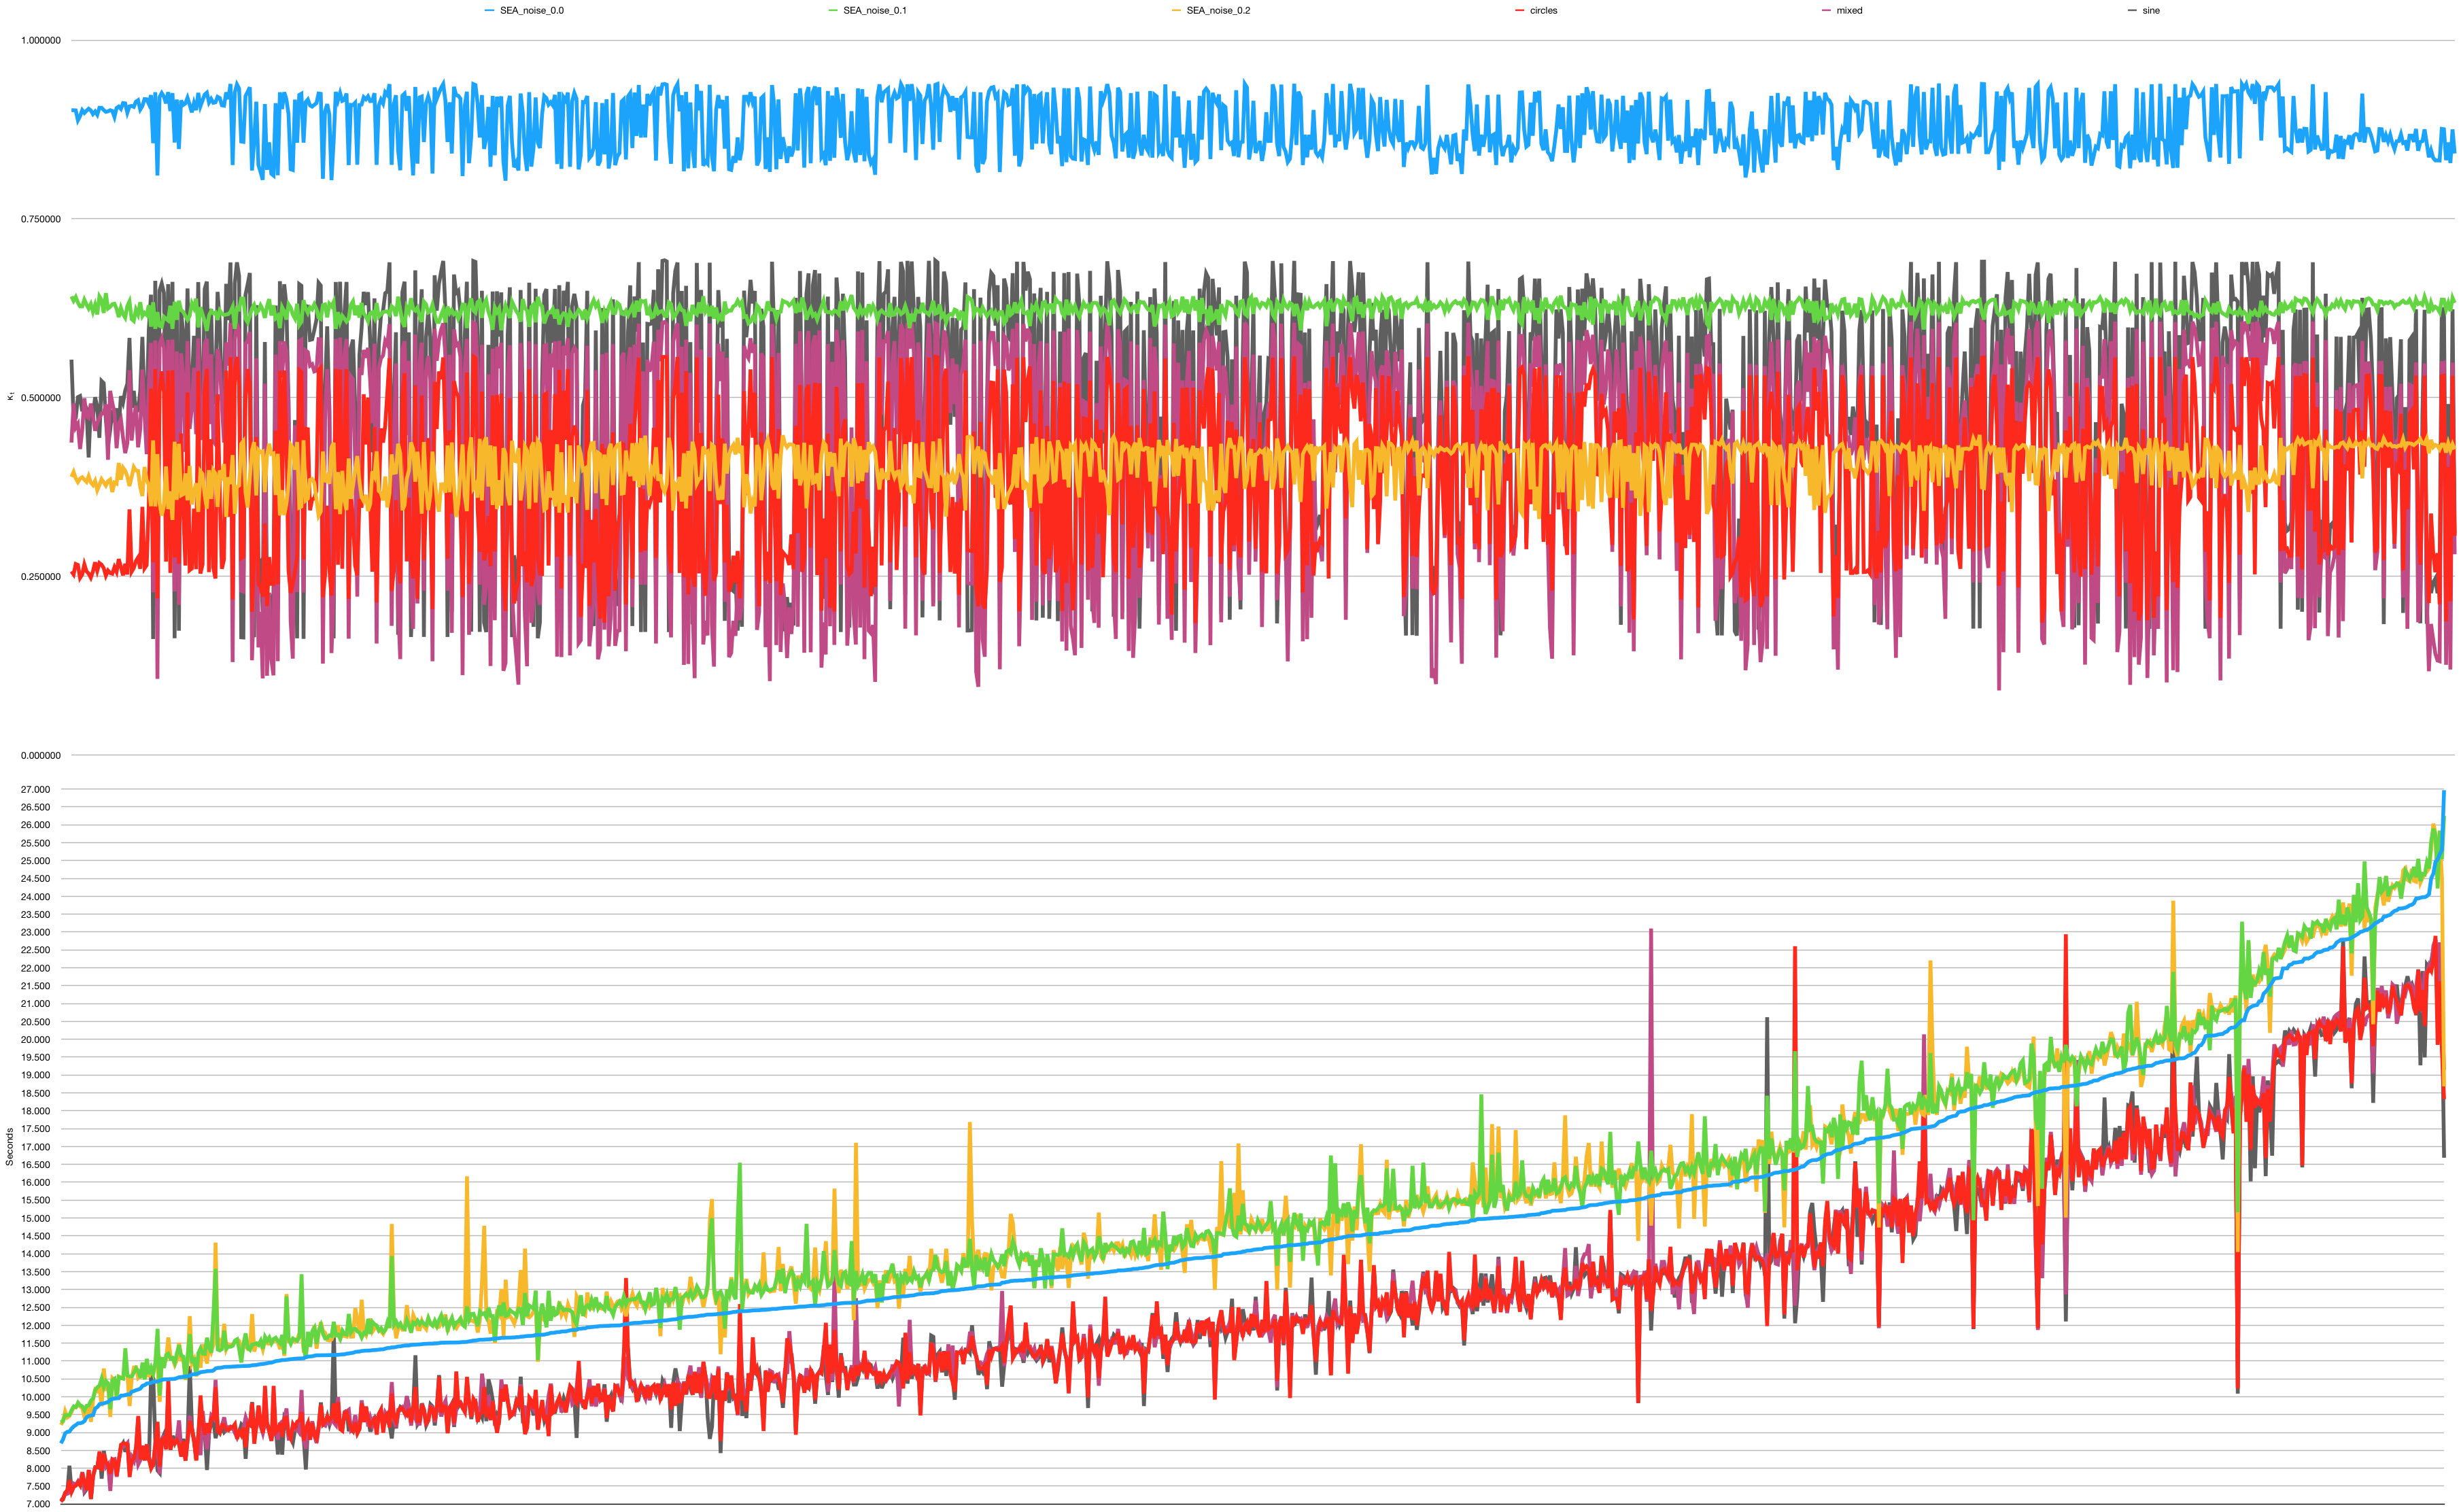
\includegraphics[width=\linewidth]{./images/chapter5/kappa_vs_time}
\caption{\label{fig:kappa_vs_time}$\kappa_t$ in relation to time, across all parameter combinations}
\end{sidewaysfigure}
Figure \ref{fig:kappa_vs_time} shows that as the execution time increases, $\kappa_t$ stays roughly constant. The majority of the changes seem to be due to the various parameter combinations. This is a good sign as it suggests that the predictive accuracy of our model is at most very loosely tied to the execution time of its algorithm.

\section{Investigating how each parameter influences each metric}

\subsection{Wilcoxon tests}

\subsubsection{Drift Detector Count}

\begin{table}[]
\centering
\caption{\label{table:wilcoxon_significant}Statistically significant percentage of parameter combinations found via the Wilcoxon test}
\begin{tabular}{|l|l|l|l|l|l|}
\hline
\textbf{Parameter} & \textbf{Measure} & \textbf{0.05} & \textbf{0.01} & \textbf{0.001} & \textbf{Total} \\ \hline \hhline{======}
\multirow{2}{*}{Drift detector count} & execution time & 5\% & 6\% & 82\% & 93\% \\ \cline{2-6} 
 & $\kappa_t$ & 4\% & 1\% & 1\% & 7\% \\ \hline\hhline{======}
\multirow{2}{*}{Window type} & execution time & 1\% & 6\% & 89\% & 97\% \\ \cline{2-6} 
 & $\kappa_t$ & 7\% & 8\% & 44\% & 60\% \\ \hline
\end{tabular}
\end{table}

As indicated by table \ref{table:wilcoxon_significant}, the parameter \textit{Drift Detector Count} seems to heavily influence the execution time of the algorithm, regardless of the other parameter values. When it comes to the $\kappa_t$ metric, only 7\% of combinations proved to have statistically significant differences in predictive performance. 

\begin{table}[]
\centering
\caption{\label{table:wilcoxon_drift_detector_count}Statistically significant percentage of parameter combinations by parameter value for Drift Detector Count found via the Wilcoxon test}
\begin{tabular}{|l|l|l|l|l|l|l|l|l|}
\hline
\multirow{3}{*}{\textbf{Measure}} & \multicolumn{4}{l|}{\textbf{1 for ensemble}} & \multicolumn{4}{l|}{\textbf{1 per classifier}} \\ \cline{2-9} 
 & \multicolumn{2}{l|}{\textbf{significant}} & \multicolumn{2}{l|}{\textbf{insignificant}} & \multicolumn{2}{l|}{\textbf{significant}} & \multicolumn{2}{l|}{\textbf{insignificant}} \\ \cline{2-9} 
 & \textbf{count} & \textbf{\%} & \textbf{count} & \textbf{\%} & \textbf{count} & \textbf{\%} & \textbf{count} & \% \\ \hline \hhline{=========}
execution time & 447 & 99\% & 22 & 73\% & 4 & 0\% & 8 & 26\% \\ \hline
$\kappa_t$ & 19 & 59\% & 206 & 48\% & 13 & 40\% & 217 & 51\% \\ \hline
\end{tabular}
\end{table}


\begin{figure}
\centering
  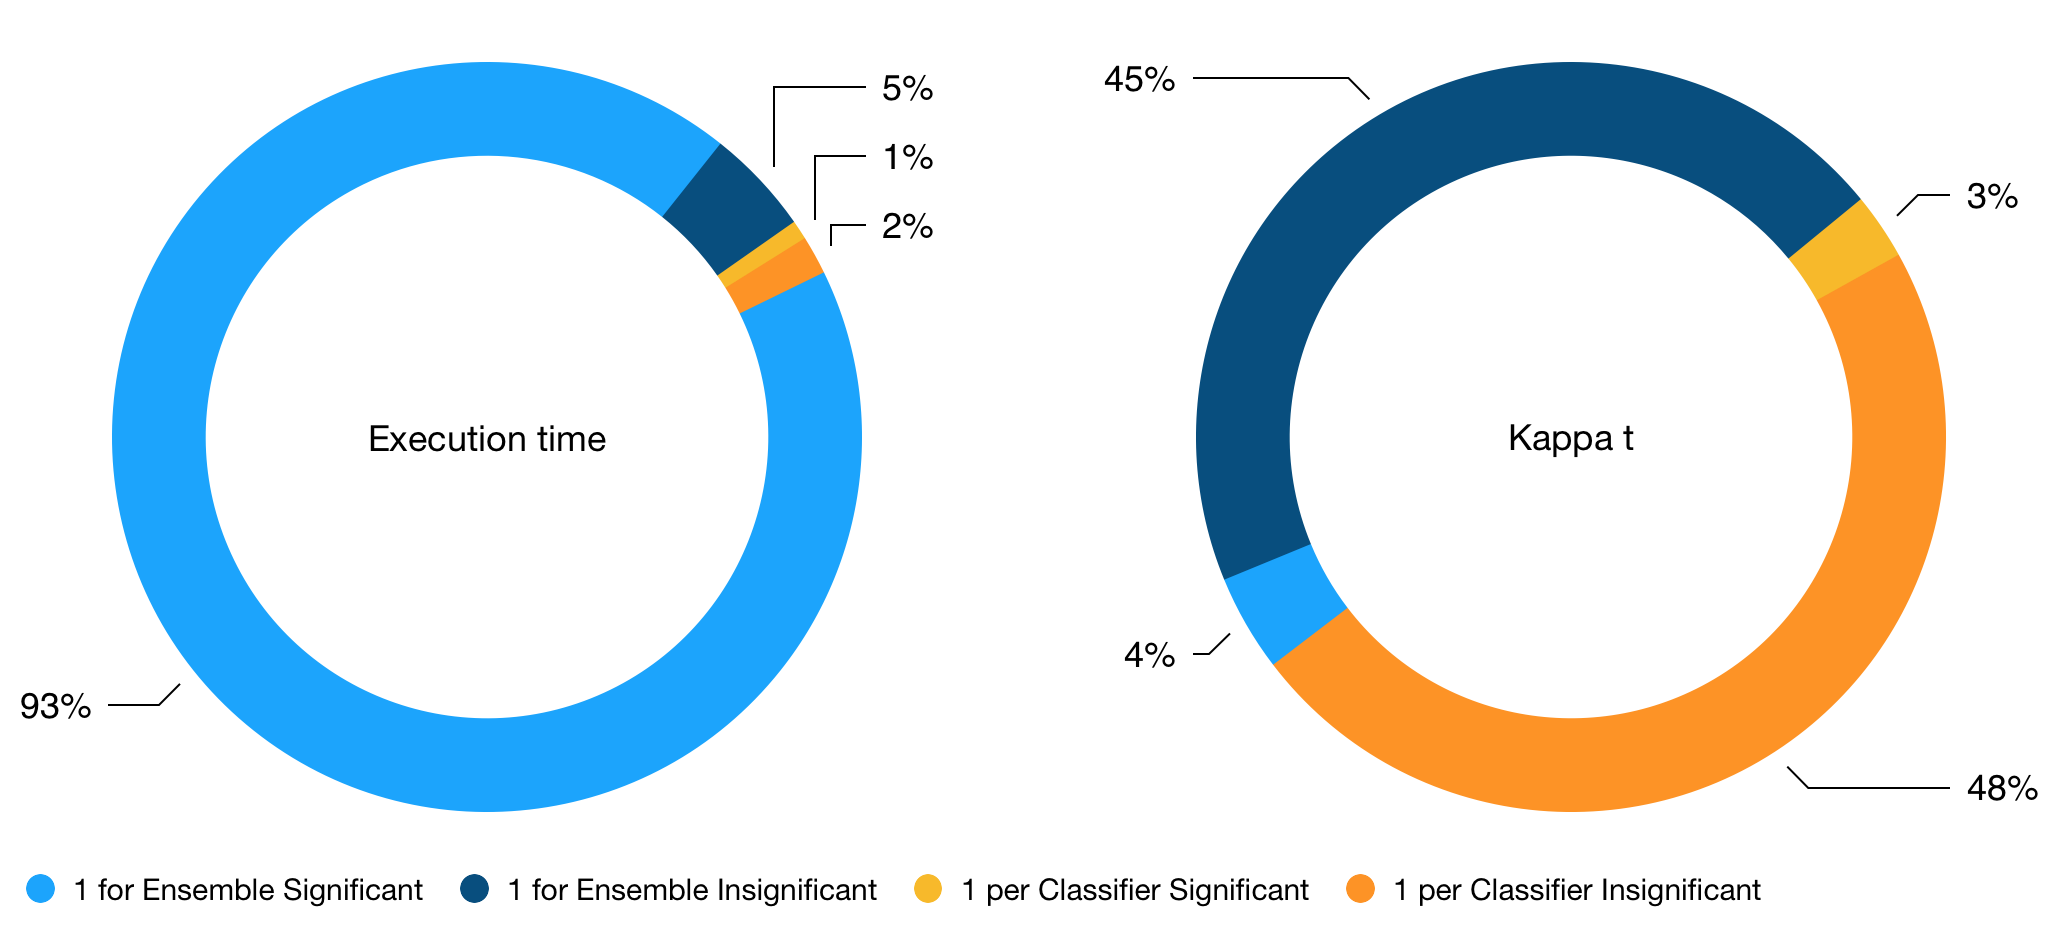
\includegraphics[width=\linewidth]{./images/chapter5/wilcoxon_drift_detector_count_pie}
\caption{\label{fig:wilcoxon_drift_detector_count_pie}Pie chart illustrating table \ref{table:wilcoxon_significant}}
\end{figure}



When we dig deeper into the \textit{Drift Detector Count} parameter, according to table \ref{table:wilcoxon_drift_detector_count} and figure \ref{fig:wilcoxon_drift_detector_count_pie}, for the execution time metric, the parameter value \textit{1 for ensemble} is evidently the best choice as it ranks best across 92\% of parameter combinations, and best across 99\% of statistically significant different results. For the $\kappa_t$ metric, it is not as clear cut; both \textit{1 for ensemble} and \textit{1 per classifier} rank best among about 50\% of the time. 

The results we found lead us to believe that choosing the \textit{1 for ensemble} value for the \textit{Drift Detector Count} parameter is very beneficial in reducing the execution time of the algorithm. While this finding might not hold across other data streams, it is likely that choosing this value for the parameter will decrease execution time significantly. Logically, it makes perfect sense that choosing \textit{1 for ensemble} over \textit{1 per classifier} leads to lower execution time because the implementation of the former is such that it performs only a fraction of the operations of the latter. Additionally, we also found that none of the parameter values consistently outranked the others in predictive accuracy, and we, therefore, cannot say if choosing a particular parameter value will result in better values for the $\kappa_t$ metric. We will later be considering the raw values to determine if a particular drift detector count leads to better predictive accuracy.

\subsubsection{Window Type}
As for the \textit{Window Type} parameter, $97\%$ of parameter combinations show a significant statistical difference in the execution time depending on the value of the window type. This indicates that the parameter value heavily influences the execution time of the algorithm, independently of other parameter values. When it comes to the $\kappa_t$ metric, over half (60\%) of combinations proved to show a statistically significant difference in predictive performance. This suggests that the \textit{Window Type} parameter could have some non-negligible influence over the $\kappa_t$ metric.

\begin{table}[]
\centering
\caption{\label{table:wilcoxon_window_type}Statistically significant percentage of parameter combinations by parameter value for Window Type found via the Wilcoxon test}
\begin{tabular}{|l|l|l|l|l|l|l|l|l|}
\hline
\multirow{3}{*}{\textbf{Measure}} & \multicolumn{4}{l|}{\textbf{Hybrid}} & \multicolumn{4}{l|}{\textbf{Sliding}} \\ \cline{2-9} 
 & \multicolumn{2}{l|}{\textbf{significant}} & \multicolumn{2}{l|}{\textbf{insignificant}} & \multicolumn{2}{l|}{\textbf{significant}} & \multicolumn{2}{l|}{\textbf{insignificant}} \\ \cline{2-9} 
 & \textbf{count} & \textbf{\%} & \textbf{count} & \textbf{\%} & \textbf{count} & \textbf{\%} & \textbf{count} & \% \\ \hline \hhline{=========}
execution time & 514 & 99\% & 6 & 54\% & 5 & 0\% & 5 & 45\% \\ \hline
$\kappa_t$ & 9 & 2\% & 86 & 40\% & 319 & 97\% & 125 & 59\% \\ \hline
\end{tabular}
\end{table}


\begin{figure}
  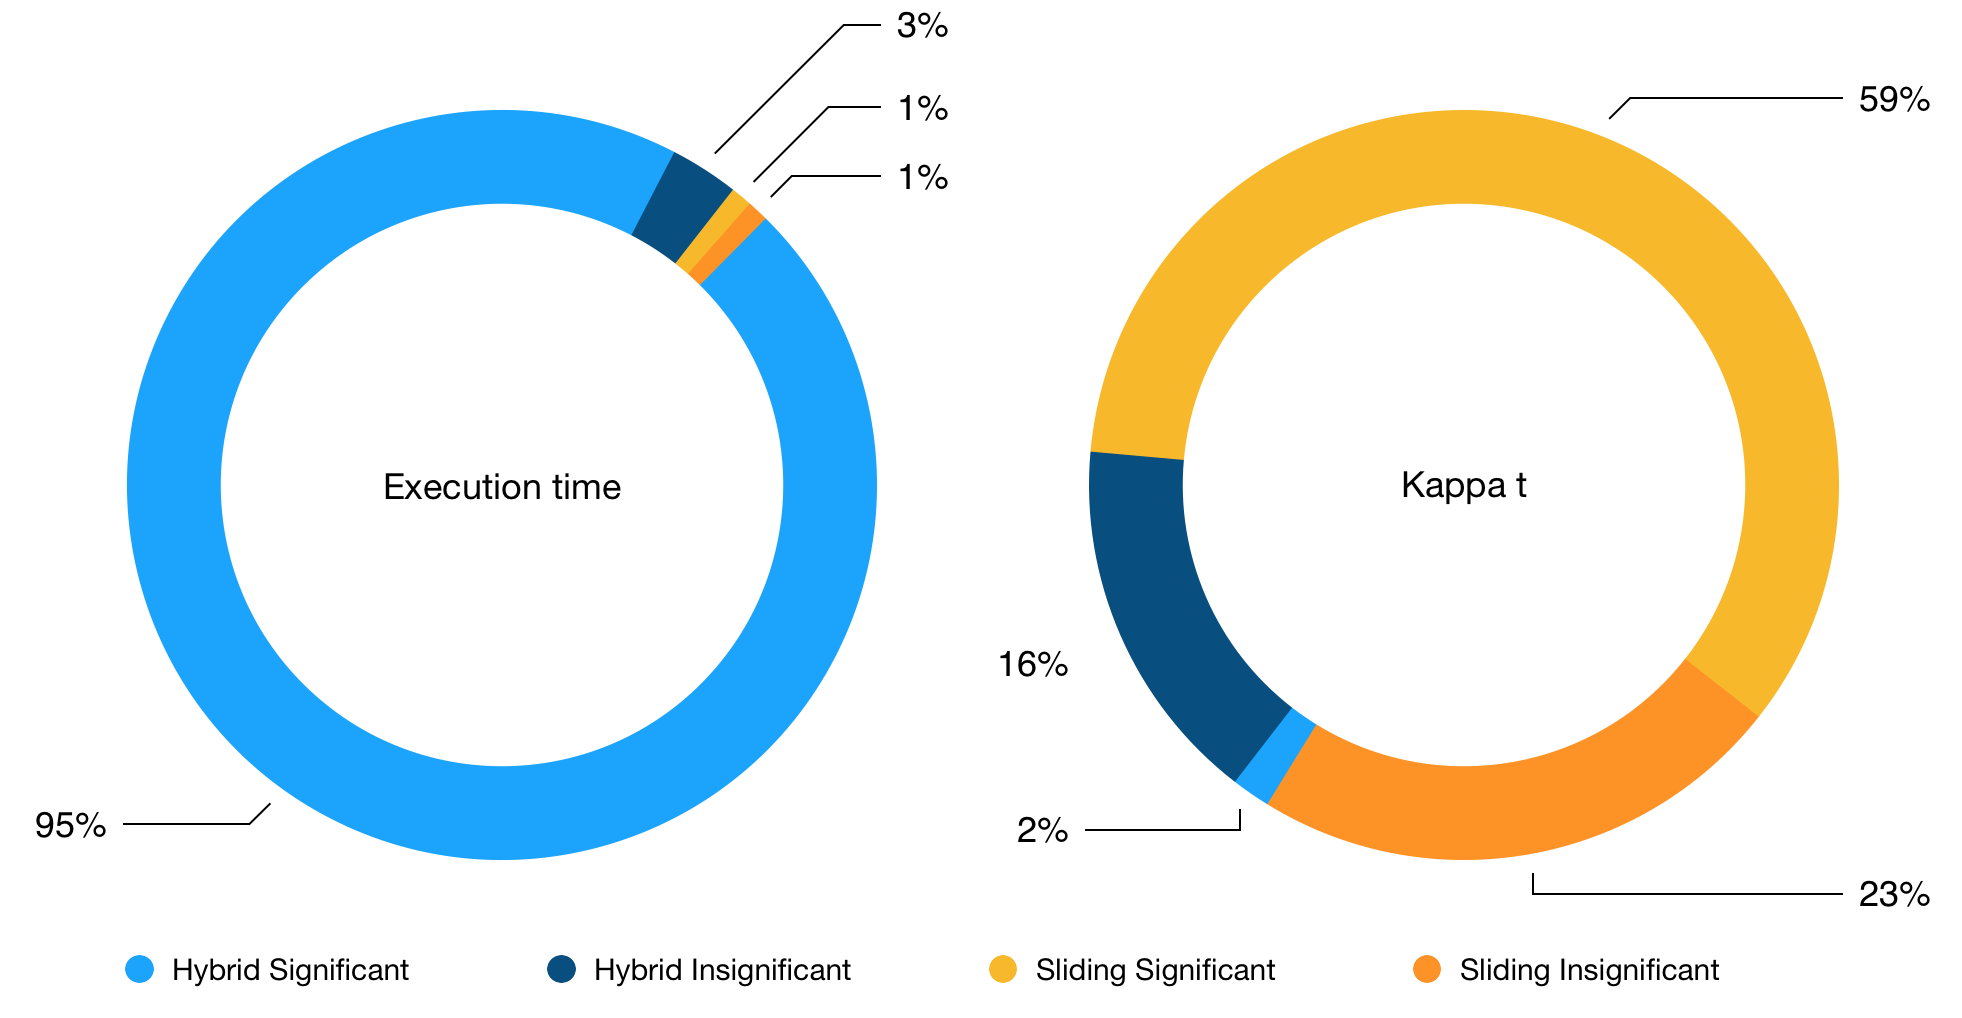
\includegraphics[width=\linewidth]{./images/chapter5/wilcoxon_window_type_pie}
\caption{\label{fig:wilcoxon_window_type_pie}Pie chart illustrating table \ref{table:wilcoxon_window_type}}
\end{figure}


When we dig deeper into the \textit{Window Type} parameter, as table \ref{table:wilcoxon_window_type} and figure \ref{fig:wilcoxon_window_type_pie} illustrates, for the execution time metric, \textit{hybrid} is evidently the best choice as it ranks best across 98\% of parameter combinations. For the $\kappa_t$ metric, it is just as obvious as \textit{sliding} ranks best across about 82\% of the parameter combinations. 

The \textit{Window Type} parameter ranking results suggest that \textit{hybrid windowing} has a significant impact on the execution time of the algorithm, independently of other parameters values. This suggests that choosing the \textit{hybrid windowing} value for the \textit{Window Type} parameter could be very beneficial in reducing the execution time of the algorithm. Again, this is exactly as expected: the implementation of \textit{hybrid windowing} is such that each sub-classifier in the ensemble only trains on each instance once, whereas the \textit{sliding windowing} technique is implemented such that each sub-classifier in the ensemble trains on each instance at least once. This, logically, leads to fewer operations, and therefore a reduction in execution time for the algorithm. This should hold true across all data streams, and therefore we recommend anyone who chooses to run this algorithm with the intent of reducing the execution time to choose the \textit{hybrid windowing} parameter value.
However, we also found that \textit{sliding windowing} outperforms \textit{hybrid windowing} across most parameter combinations, with or without a significant statistical difference. Again, using the explanation above for the reduction in execution time, since each sub-classifier training using \textit{sliding windowing} trains on each instance multiple times, it is logical that it is better able to fit the data instance in its model. 
This means that the algorithm presents a trade-off between execution time and predictive accuracy when considering the \textit{Window Type} parameter. Whoever runs the algorithm must choose which metric they value more, and choose a windowing type accordingly.

As other parameters can take more than two values, we must use the Friedman test in combination with the post-hoc Nemenyi test in order to test our null hypotheses.

\subsection{Post-hoc Nemenyi tests}

\begin{table}[]
\centering
\caption{\label{table:nemenyi_significant_breakdown}Percentage of parameter combinations that showed statistically significant differences from the post-hoc Nemenyi test}
\begin{tabular}{|l|l|c|l|c|l|}
\hline
\textbf{Parameter} & \textbf{Measure} & \textbf{Significant} & \textbf{\%} & \textbf{Insignificant} & \textbf{\%} \\ \hline \hhline{======}
\multirow{2}{*}{Batch size} & $\kappa_t$ & $\frac{1}{330}$ & $0.3\%$ & $\frac{229}{330}$ & $99.70\%$ \\ \cline{2-6} 
 & execution time & $\frac{287}{330}$ & $86.97\%$ & $\frac{43}{330}$ & $13.03\%$ \\ \hline \hhline{======}
\multirow{2}{*}{Drift reset type} & $\kappa_t$ & $\frac{1}{330}$ & $0.30\%$ & $\frac{329}{330}$ & $99.70\%$ \\ \cline{2-6} 
 & execution time & $\frac{64}{330}$ & $19.39\%$ & $\frac{266}{330}$ & $80.61\%$ \\ \hline \hhline{======}
\multirow{2}{*}{Ground truth} & $\kappa_t$ & $\frac{57}{198}$ & $28.79\%$ & $\frac{141}{198}$ & $71.21\%$ \\ \cline{2-6} 
 & execution time & $\frac{168}{198}$ & $84.85\%$ & $\frac{30}{198}$ & $15.15\%$ \\ \hline \hhline{======}
\multirow{2}{*}{Voting type} & $\kappa_t$ & $\frac{0}{180}$ & $0\%$ & $\frac{180}{180}$ & $100.00\%$ \\ \cline{2-6} 
 & execution time & $\frac{154}{180}$ & $85.56\%$ & $\frac{26}{180}$ & $14.44\%$ \\ \hline
\end{tabular}
\end{table}

\begin{table}[]
\centering
\caption{\label{table:nemenyi_significant_breakdown_aggregate}Number of different ranking and statistically significant parameter combinations from table \ref{table:nemenyi_significant_breakdown}}
\begin{tabular}{|l|l|c|c|}
\hline
\textbf{Parameter} & \textbf{Measure} & \textbf{Significant} & \textbf{Insignificant} \\ \hline \hhline{====}
\multirow{2}{*}{Batch size} & $\kappa_t$ & $ 1 \rightarrow 1 $ & $ 229 \rightarrow 6 $ \\ \cline{2-4} 
 & execution time & $ 287 \rightarrow 2 $ & $ 43 \rightarrow 2 $ \\ \hline \hhline{====}
\multirow{2}{*}{Drift reset type} & $\kappa_t$ & $ 1 \rightarrow 1 $ & $ 229 \rightarrow 6 $ \\ \cline{2-4} 
 & execution time & $ 64 \rightarrow 6 $ & $ 266 \rightarrow 6 $ \\ \hline \hhline{====}
\multirow{2}{*}{Ground truth} & $\kappa_t$ & $ 57 \rightarrow 3 $ & $ 141 \rightarrow 6 $ \\ \cline{2-4} 
 & execution time & $ 168 \rightarrow 22 $ & $ 30 \rightarrow 16 $ \\ \hline \hhline{====}
\multirow{2}{*}{Voting type} & $\kappa_t$ & $ 0 \rightarrow 0 $ & $ 180 \rightarrow 4 $ \\ \cline{2-4} 
 & execution time & $ 154 \rightarrow 2 $ & $ 26 \rightarrow 3 $ \\ \hline
\end{tabular}
\end{table}

\subsubsection{Batch Size}

As we can observe from table \ref{table:nemenyi_significant_breakdown}, only one combination of parameters among 330 were significantly statistically different when considering the $\kappa_t$ metric for the batch size parameter, which is a negligible amount. As for the execution time metric, almost $87\%$ of parameter combinations proved to show a significant statistical difference. This confirms our expectations that changing only the batch size has a significant impact on the execution time of the algorithm but no significant impact on its predictive accuracy.
The first row of table \ref{table:nemenyi_significant_breakdown_aggregate} indicates that there are seven variations of rankings of batch size rankings for the $\kappa_t$ metric; the second line indicates that there are two variations of rankings and pairs of parameters that were significantly statistically different and two variations of ranks for batch sizes that were insignificant. These values are illustrated in table \ref{table:batch_size_rankings} and figure \ref{fig:batch_size_rankings_pie}.

\begin{table}[]
\centering
\caption{\label{table:batch_size_rankings}Rankings for batch size and parameter combination counts}
\begin{tabular}{|l|c|l|c|c|}
\hline
\textbf{Metric} & \textbf{Stat. Sig.} & \textbf{Ranks} & \textbf{Stat. Sig. values} & \textbf{\%} \\ \hline \hhline{=====}
\multirow{7}{*}{$\kappa_t$} & \checkmark & 25 / 75 / 100 & 25 / 100 & 0.30\% \\ \cline{2-5} 
 & \multirow{6}{*}{$\times$} & 100 / 25 / 75 & \multirow{6}{*}{} & 16.36\% \\ \cline{3-3} \cline{5-5} 
 &  & 100 / 75 / 25 &  & 10.30\% \\ \cline{3-3} \cline{5-5} 
 &  & 25 / 100 / 75 &  & 16.67\% \\ \cline{3-3} \cline{5-5} 
 &  & 25 / 75 / 100 &  & 27.58\% \\ \cline{3-3} \cline{5-5} 
 &  & 75 / 100 / 25 &  & 10.00\% \\ \cline{3-3} \cline{5-5} 
 &  & 75 / 25 / 100 &  & 18.79\% \\ \hline \hhline{=====}
\multirow{4}{*}{Execution time} & \multirow{2}{*}{\checkmark} & 100 / 75 / 25 & 100 / 25 & 71.52\% \\ \cline{3-5} 
 &  & 75 / 100 / 25 & 75 / 25 & 15.45\% \\ \cline{2-5} 
 & \multirow{2}{*}{$\times$} & 100 / 75 / 25 & \multirow{2}{*}{} & 6.67\% \\ \cline{3-3} \cline{5-5} 
 &  & 75 / 100 / 25 &  & 6.36\% \\ \hline
\end{tabular}
\end{table}

\begin{figure}
  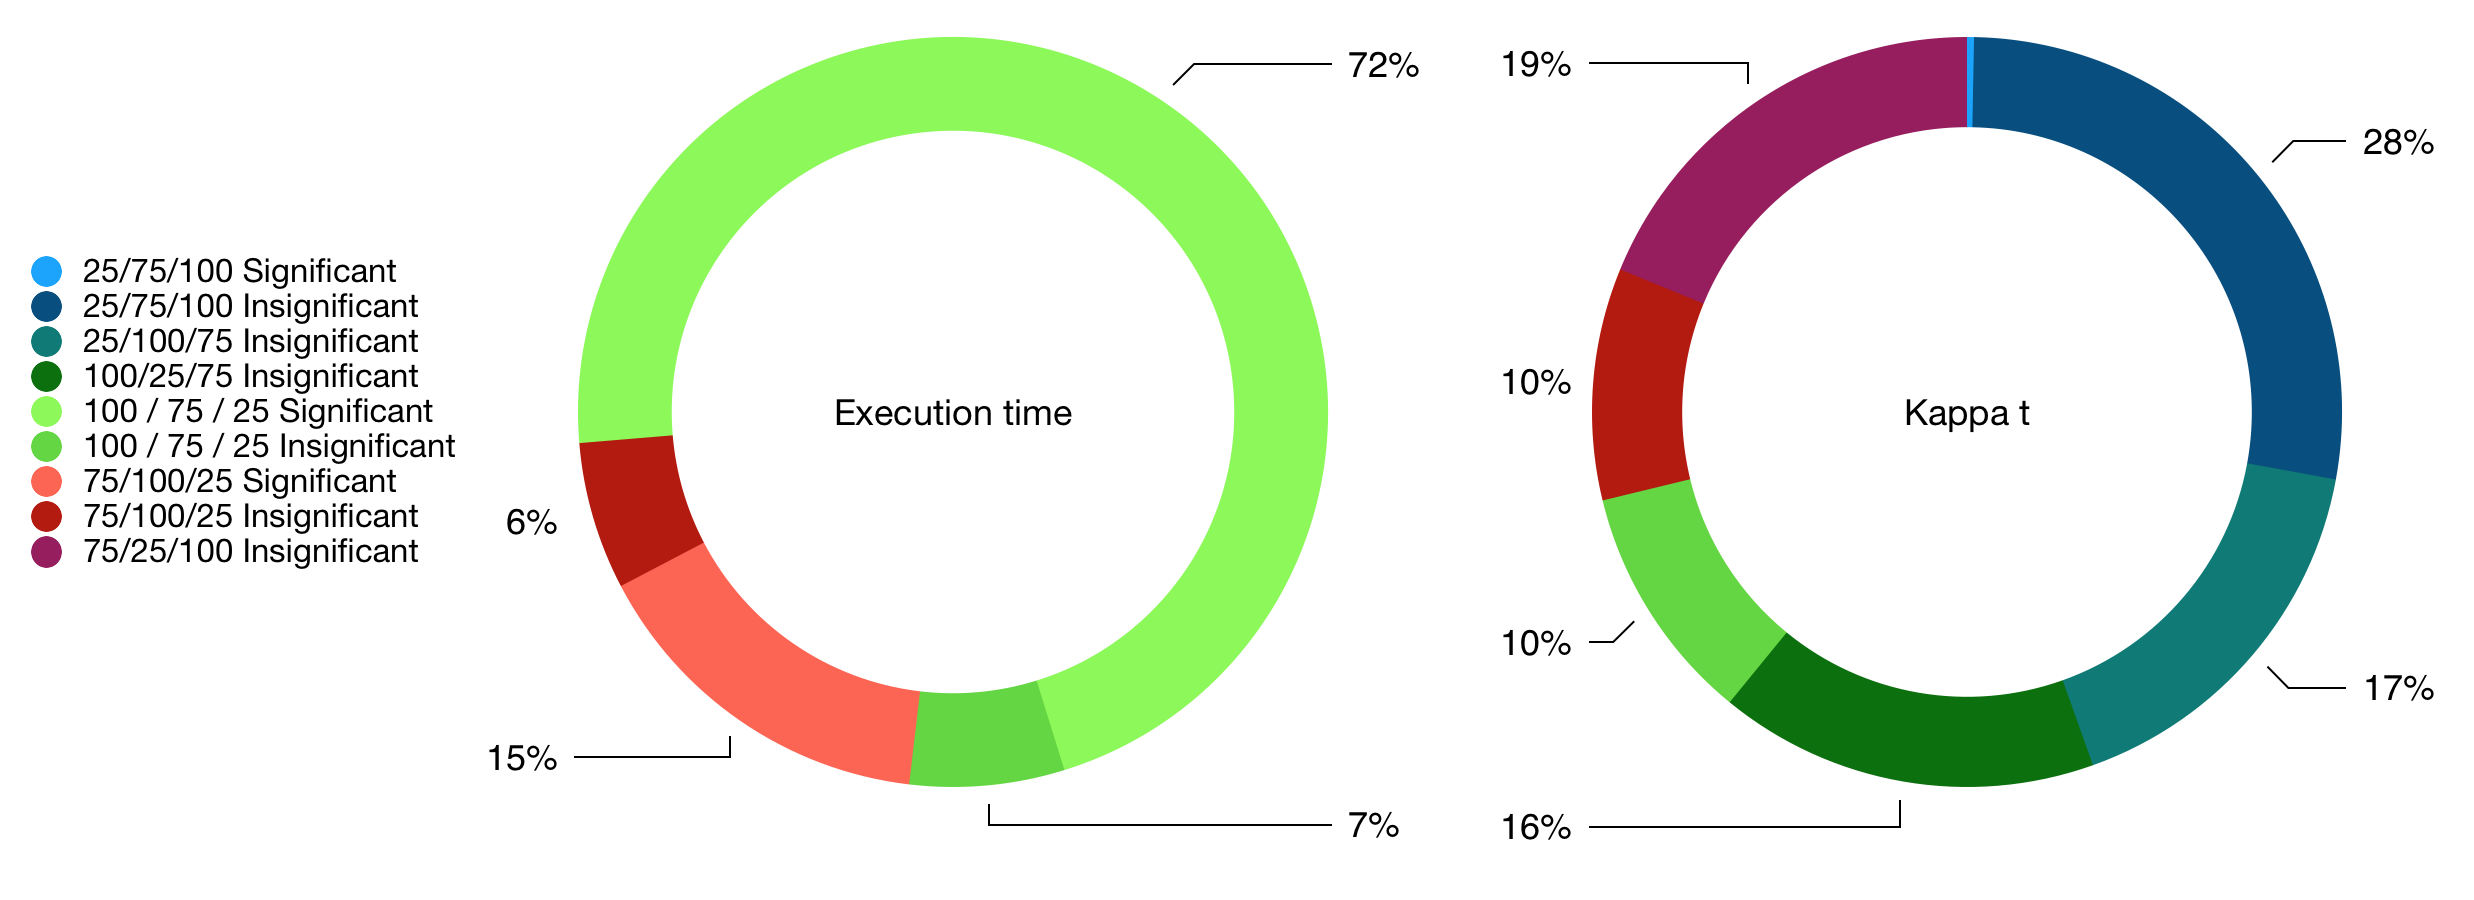
\includegraphics[width=\linewidth]{./images/chapter5/batch_size_rankings_pie}
\caption{\label{fig:batch_size_rankings_pie}Pie chart illustrating table \ref{table:batch_size_rankings}}
\end{figure}

Let us examine the pie charts illustrating the rankings of the \textit{Batch size} parameter values.
We will first examine the results for the execution time. At first glance, we notice that \textit{100} clearly ranks first over the majority of parameter combinations, followed by \textit{75} over a minority of combinations.
For the $\kappa_t$ metric, the rankings are less clear. \textit{25} seems to rank first more frequently (across $45\%$ of parameter combinations), whereas \textit{75} and \textit{100} rank first across $26\%$ of parameter combinations each. These rankings do not tell us how much the difference is across parameter combinations. By this, we mean that while a parameter value may rank first across a larger percentage of parameter combinations, it may actually perform worse than another value over a smaller percentage of parameter combinations.
In any case, the results indicate that there is another trade-off to be made in regards to the batch size parameter between predictive accuracy and execution time. Again, we expected these results as a batch size of 100 allows the ensemble to learn from more examples at once, which reduces the number of operations that would have to be repeated were we to use a batch size of 25 for example, where each operation down the line would be run 4 times instead of only 1 time. As for predictive accuracy, \textit{25} has a slight advantage over the other parameter values possibly because there is a better chance that a drift wreaks havoc on a sub-classifier's ability to train on a batch of \textit{75} or \textit{100} than on a batch of \textit{25}. For a batch of \textit{25}, the sub-classifiers can be reset sooner, and the next batch may be easier to model.

\subsubsection{Drift Reset Type}

Let us now investigate the Drift Reset Type parameter. In table \ref{table:nemenyi_significant_breakdown}, only a single out of 330 parameter combinations showed a significant statistical difference in parameter values when considering the $\kappa_t$ metric, whereas about $20\%$ of parameter values showed a statistically significant difference in parameter values when considering the execution time metric. This suggests that the value of the drift reset type parameter does not have a significant impact over other values on the measured metrics.
Table \ref{table:nemenyi_significant_breakdown_aggregate}, lists the number of different rankings found in table \ref{table:drift_reset_type_rankings} over the measured metrics, depending on whether results showed a statistical significant difference.

Let us examine table \ref{table:drift_reset_type_rankings} or better yet, the pie charts shown in figure \ref{fig:drift_reset_type_rankings_pie} illustrating the rankings of the \textit{Drift Reset Type} parameter values.
Again, we will first examine the results for the execution time. At first glance, we notice that \textit{blind resets} clearly ranks first the least over the parameter combinations. \textit{Reset all} ranks first across half of the parameter combinations and \textit{partial resets} over about a third of them. This is a good sign, and expected. Since sub-classifiers must be reset more frequently, they must be completely re-trained on data, which also prevents them from learning from a larger set of older data. This might be good for streams with very frequent drifts, but those where they infrequently appear, blindly resetting the classifier prevents it from remembering possibly useful historical data.

For the $\kappa_t$ metric, the rankings are not as clear. Again, we must remember that these rankings do not tell us the difference across parameter combinations, meaning that while a parameter value may rank first across a more significant percentage of parameter combinations, it may perform less well than another value over a smaller percentage of parameter combinations.
In any case, the results indicate that each parameter value ranks first across a third of parameter combinations. This does not allow us to conclude much, other than blind resets may perform just as well as resetting every sub-classifier or only a minority of them. It could be that the sub-classifiers are not very apt at learning from the data, or that resetting the sub-classifiers is not very useful. Another reason could be attributed to the way partial drift resets work, in that each sub-classifier has a chance of being reset, meaning that there is a chance that the offending sub-classifier that is not correctly adapting to the concept drift is not reset. A more thorough investigation is unfortunately outside of the scope of this work, due to time constraints. It could also be that the predictive accuracy cannot improve much after a drift due to the limitations of the sub-classifiers to model the data effectively. Either way, this is truly unfortunate, as it suggests that changing how often and how many sub-classifiers are reset does not seem to affect the $\kappa_t$ metric.
These results indicate that blind resets perform almost as well as our other reset strategies, which may suggest that our drift reset strategy needs further investigation.

\begin{table}[]
\centering
\caption{\label{table:drift_reset_type_rankings}Rankings for drift reset type and parameter combination counts}
\begin{tabular}{|l|c|l|c|c|}
\hline
\textbf{Metric} & \textbf{Stat. Sig.} & \textbf{Ranks} & \textbf{Stat. Sig. values} & \textbf{\%} \\ \hline \hhline{=====}
\multirow{7}{*}{$\kappa_t$} & \checkmark & BLIND / ALL / PARTIAL & BLIND / PARTIAL & 0.30\% \\ \cline{2-5}
 & \multirow{6}{*}{$\times$} & ALL / BLIND / PARTIAL & \multirow{6}{*}{} & 23.64\% \\ \cline{3-3} \cline{5-5} 
 &  & ALL / PARTIAL / BLIND &  & 13.64\% \\ \cline{3-3} \cline{5-5} 
 &  & BLIND / ALL / PARTIAL &  & 15.45\% \\ \cline{3-3} \cline{5-5} 
 &  & BLIND / PARTIAL / ALL &  & 17.88\% \\ \cline{3-3} \cline{5-5} 
 &  & PARTIAL / ALL / BLIND &  & 14.24\% \\ \cline{3-3} \cline{5-5} 
 &  & PARTIAL / BLIND / ALL &  & 14.85\% \\ \hline \hhline{=====}
\multirow{12}{2cm}{Execution time} & \multirow{6}{*}{\checkmark} & ALL / PARTIAL / BLIND & ALL / BLIND & 6.97\% \\ \cline{3-5} 
 &  & ALL / BLIND / PARTIAL & ALL / PARTIAL & 0.61\% \\ \cline{3-5} 
 &  & BLIND / PARTIAL / ALL & BLIND / ALL & 0.91\% \\ \cline{3-5} 
 &  & BLIND / ALL / PARTIAL & BLIND / PARTIAL & 0.91\% \\ \cline{3-5} 
 &  & PARTIAL / BLIND / ALL & PARTIAL / ALL & 1.52\% \\ \cline{3-5} 
 &  & PARTIAL / ALL / BLIND & PARTIAL / BLIND & 8.48\% \\ \cline{2-5} 
 & \multirow{6}{*}{$\times$} & ALL / BLIND / PARTIAL & \multirow{6}{*}{} & 6.36\% \\ \cline{3-3} \cline{5-5} 
 &  & ALL / PARTIAL / BLIND &  & 36.36\% \\ \cline{3-3} \cline{5-5} 
 &  & BLIND / ALL / PARTIAL &  & 7.58\% \\ \cline{3-3} \cline{5-5} 
 &  & BLIND / PARTIAL / ALL &  & 5.45\% \\ \cline{3-3} \cline{5-5} 
 &  & PARTIAL / ALL / BLIND &  & 21.82\% \\ \cline{3-3} \cline{5-5} 
 &  & PARTIAL / BLIND / ALL &  & 3.03\% \\ \hline
\end{tabular}
\end{table}

\begin{figure}
  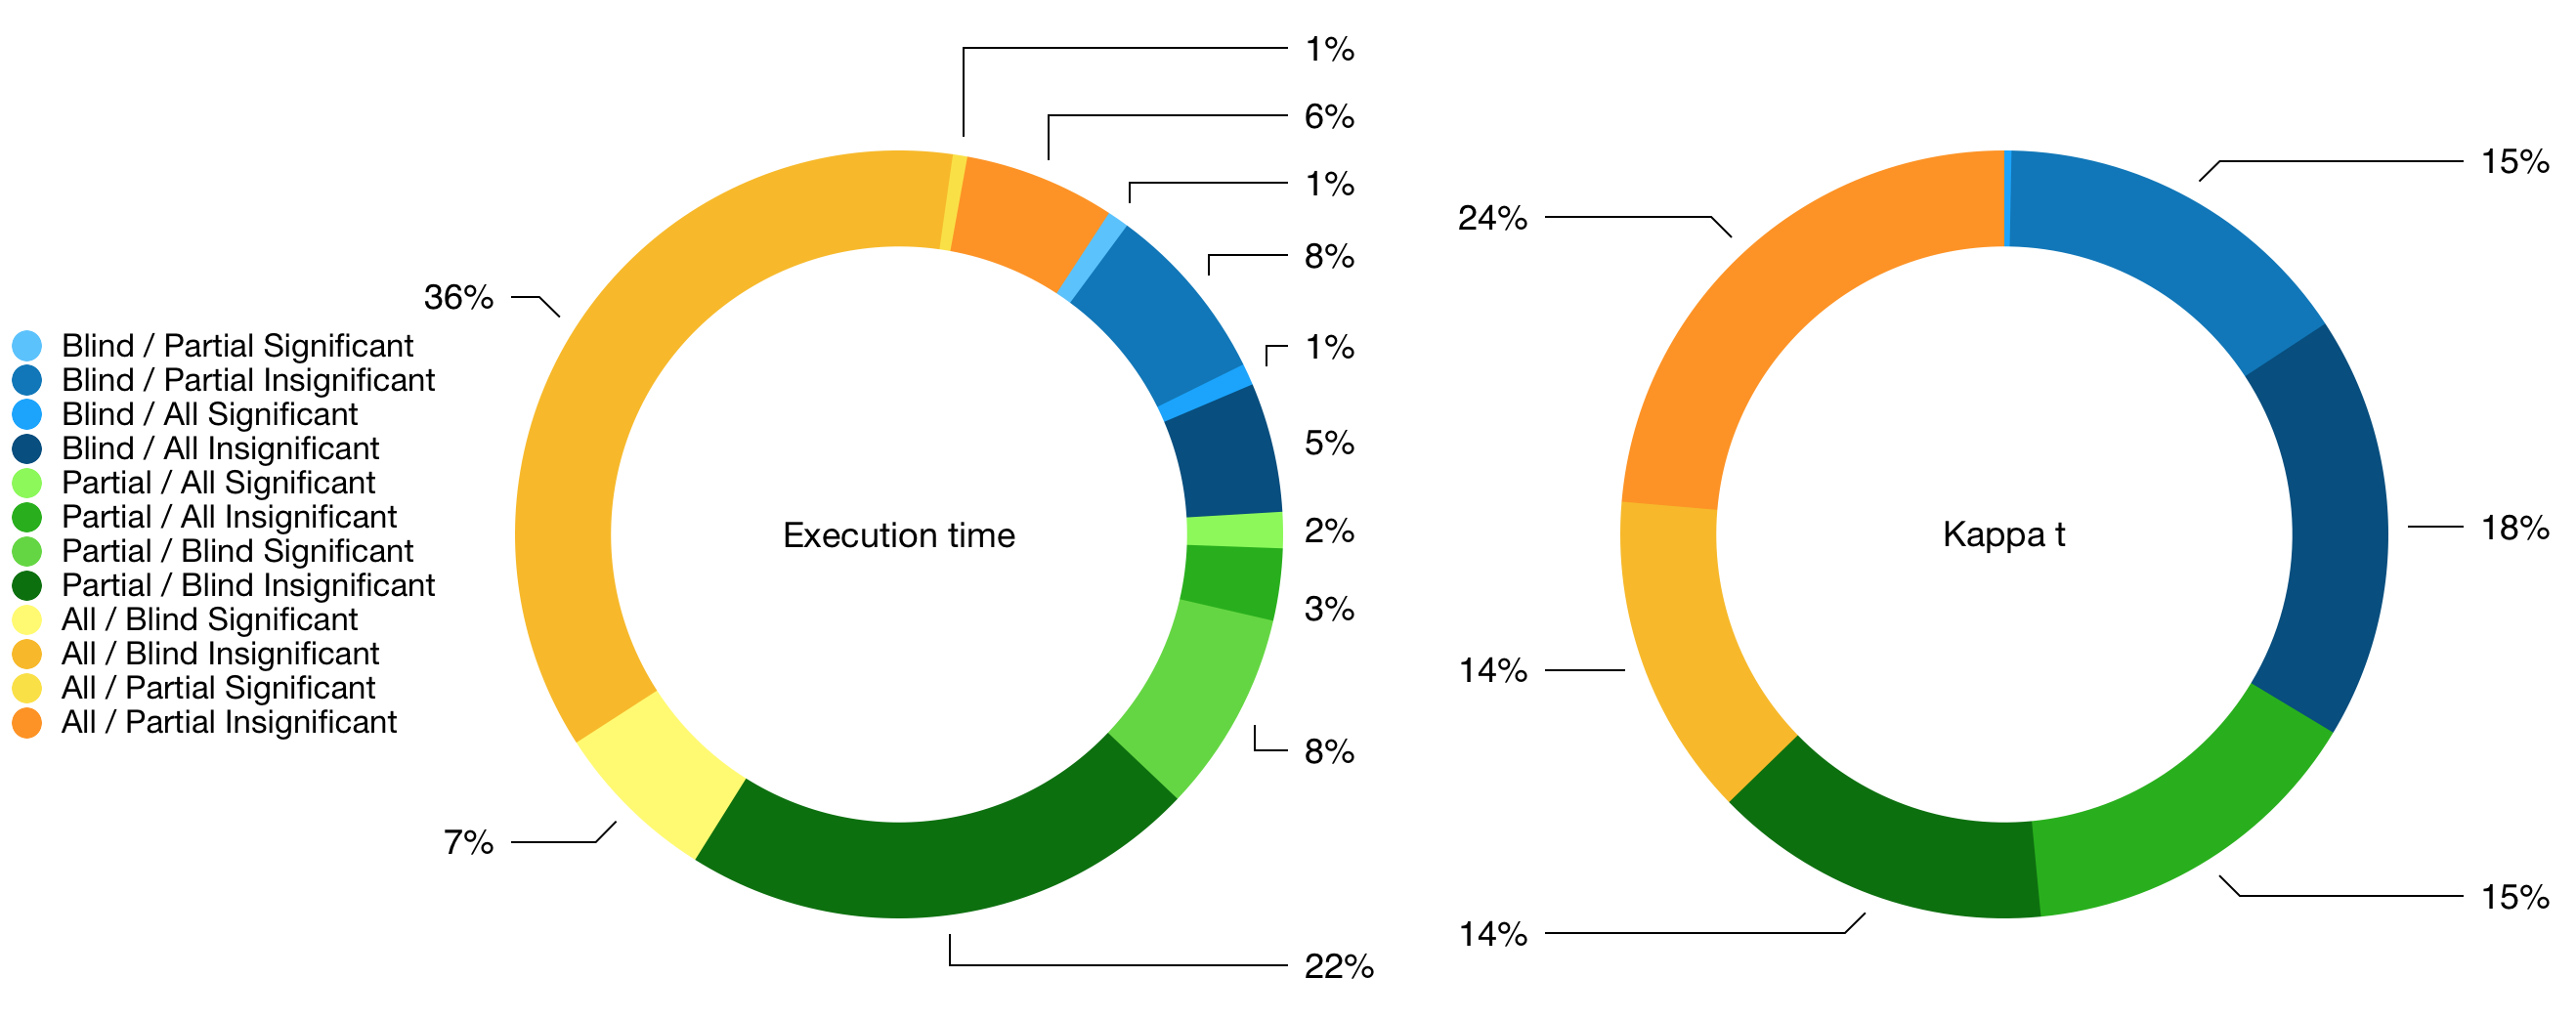
\includegraphics[width=\linewidth]{./images/chapter5/drift_reset_type_rankings_pie}
\caption{\label{fig:drift_reset_type_rankings_pie}Pie chart illustrating table \ref{table:drift_reset_type_rankings}}
\end{figure}

\subsubsection{Ground Truth}

Let us now investigate the Ground Truth parameter (which indicates the percentage of labelled instances used to train our ensemble). Table \ref{table:nemenyi_significant_breakdown} shows that less than one-third of parameter combinations show a statistically significant difference for the $\kappa_t$ metric; but over $84\%$ for the execution time metric. This suggests that the value of the ground truth parameter has a measurable impact on the execution time, across a large portion of the other parameters, (almost) no matter their values.

Table \ref{table:ground_truth_rankings} shows that, for the $\kappa_t$ metric, there are multiple possible options for ranking the parameter values. For those with a statistically significant difference, 100 performs better than 60. 100 ranks first across all parameter combinations over $98\%$ of the time, as expected. This is normal, as we expect our ensemble to better learn to model the streamed data from ground truth rather than from its own predictions of class label values, considering that it can enable our ensemble to learn from erroneously labelled data. It is a good sign, however, that there is no statistically significant difference for parameter values other than 100 and 60. It is logical that selecting a higher percentage of ground truth will lead to higher predictive accuracy, but we can allow for a trade-off between predictive accuracy and time.

In table \ref{table:ground_truth_rankings}, there are different combinations for ranks and statistical significant different values for the execution time metric. Combinations with $60\%$ ground truth rank first across $74.31\%$ of parameter combinations, and $100\%$ ground truth ranks first across only $17.71\%$ of parameter values. When we exclude insignificant results, our previous observation remains true, but across a smaller percentage of parameter combinations, but only by $5\%$ to $10\%$. We can conclude that using $60\%$ ground truth is more likely to decrease execution time. This is an unexpected finding, as we expected that using less ground truth would cause an increase in execution time by causing more drift detection events and therefore more model resets and retrains. However, it is possible that by using less ground truth, there are no drift detection events because the model is not able to properly learn from the data, so the model is never reset or retrained which might also explain why this parameter value also ranks as one of the worst in predictive accuracy.

When looking at the raw values, as depicted in figure \ref{fig:order_by_ground_truth}, we notice that the $\kappa_t$ metric does not change much over the parameter combinations, but rises noticeably starting when using $80\%$ ground truth. The regular peaks and valleys within each set of ground truth values (separated by black vertical lines) represent how other parameters affect $\kappa_t$. We also notice that the amount of ground truth has a strong effect over the sine1, mixed and particularly on the circles data sets. It may be that it is easier to model the data from SEA than from the other data sets, and therefore it does not need as much ground truth to build an accurate model. Not much can be said when looking at the raw values for the execution time metric other than that there may be fewer valleys in the section dedicated for the $60\%$ ground truth parameter.

\begin{table}[]
\centering
\caption{\label{table:ground_truth_rankings}Rankings for ground truth and parameter combination counts}
\begin{tabular}{|l|c|l|c|c|}
\hline
\textbf{Metric} & \textbf{Stat. Sig.} & \textbf{Ranks} & \textbf{Stat. Sig. values} & \textbf{\%} \\ \hline
\multirow{4}{*}{$\kappa_t$} & \checkmark & 100 / x / x / x / 60 & 100 / 60 & 28.80\% \\ \cline{2-5} 
 & \multirow{3}{*}{$\times$} & 100 / x / x / x / 60 & \multirow{3}{*}{} & 65.15\% \\ \cline{3-3} \cline{5-5} 
 &  & 100 / x / x / 60 / 70 &  & 4.55\% \\ \cline{3-3} \cline{5-5} 
 &  & 80 / 100 / 90 / 70 / 60 &  & 1.52\% \\ \hline
\multirow{21}{*}{Execution time} & \multirow{12}{*}{\checkmark} & 100 / 60 / x / x / 70 & 100 / 70 & 9.10\% \\ \cline{3-5} 
 &  & 100 / 60 / 90 / 80 / 70 & \begin{tabular}[c]{@{}c@{}}100 / 70\\ 60 / 70\end{tabular} & 0.51\% \\ \cline{3-5} 
 &  & 100 / 60 / 90 / 70 / 80 & 100 / 80 & 2.02\% \\ \cline{3-5} 
 &  & 100 / 60 / 80 / 70 / 90 & 100 / 90 & 0.51\% \\ \cline{3-5} 
 &  & 60 / x / x / x / 100 & 60 / 100 & 14.16\% \\ \cline{3-5} 
 &  & 60 / x / x / x / 70 & 60 / 70 & 1.02\% \\ \cline{3-5} 
 &  & 60 / x / x / x / 80 & 60 / 80 & 50.51\% \\ \cline{3-5} 
 &  & 60 / 70 / 100 / 80 / 90 & \begin{tabular}[c]{@{}c@{}}60 / 80\\ 60 / 90\end{tabular} & 0.51\% \\ \cline{3-5} 
 &  & 60 / 80 / 70 / 100 / 90 & 60 / 90 & 1.01\% \\ \cline{3-5} 
 &  & 70 / 90 / 80 / 100 / 60 & \begin{tabular}[c]{@{}c@{}}70 / 60\\ 90 / 60\end{tabular} & 0.51\% \\ \cline{3-5} 
 &  & 90 / x / x / x / 100 & 90 / 100 & 2.03\% \\ \cline{3-5} 
 &  & 90 / 70 / 80 / 100 / 60 & 90 / 60 & 3.03\% \\ \cline{2-5} 
 & \multirow{9}{*}{$\times$} & 100 / 60 / x / x / 90 & \multirow{9}{*}{} & 1.02\% \\ \cline{3-3} \cline{5-5} 
 &  & 100 / 60 / x / x / 70 &  & 1.52\% \\ \cline{3-3} \cline{5-5} 
 &  & 100 / 60 / 90 / 70 / 80 &  & 3.03\% \\ \cline{3-3} \cline{5-5} 
 &  & 60 / x / x / 80 / 90 &  & 1.52\% \\ \cline{3-3} \cline{5-5} 
 &  & 60 / x / x / x / 80 &  & 3.55\% \\ \cline{3-3} \cline{5-5} 
 &  & 60 / 100 / 90 / 80 / 70 &  & 0.51\% \\ \cline{3-3} \cline{5-5} 
 &  & 60 / x / x / 80 / 100 &  & 1.52\% \\ \cline{3-3} \cline{5-5} 
 &  & 90 / x / x / x / 100 &  & 2.03\% \\ \cline{3-3} \cline{5-5} 
 &  & 90 / 70 / 80 / 100 / 60 &  & 0.51\% \\ \hline
\end{tabular}
\end{table}

\begin{sidewaysfigure}
  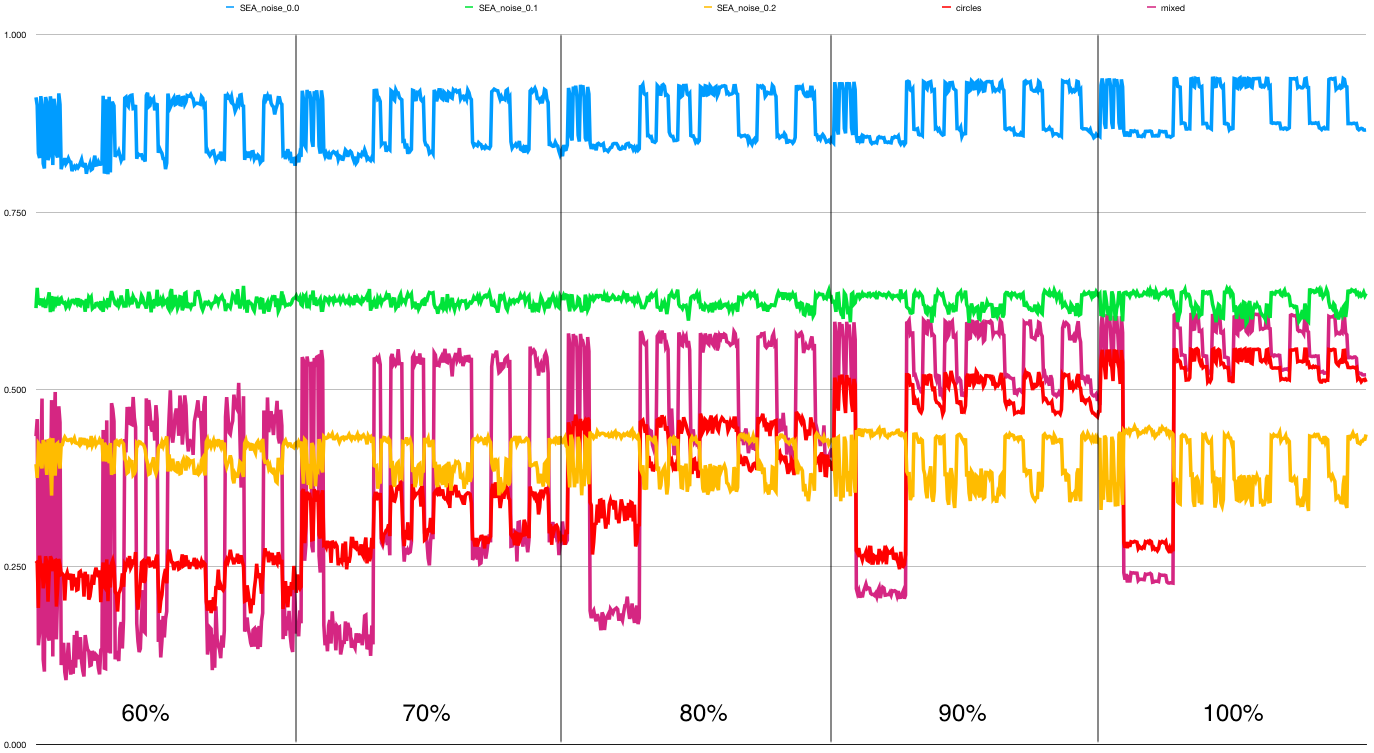
\includegraphics[width=\linewidth]{./images/chapter5/ground_truth}
\caption{\label{fig:order_by_ground_truth}$\kappa_t$ across all parameter combinations, ordered by ground truth}
\end{sidewaysfigure}

\subsubsection{Voting Type}

Finally, we investigate the Voting Type parameter. As table \ref{table:nemenyi_significant_breakdown} shows, none of the 180 parameter combinations proved to show a significant statistical difference for the $\kappa_t$ metric. However, a large portion of the parameter combinations showed a significant statistical significance for the execution time parameter ($85.56\%$ of combinations). This leads us to believe that the voting type does not have a significant influence on predictive accuracy. However, for execution time, there is a statistically significant difference present across a good majority of parameter combinations, leading us to believe that the significance remains true across a good portion of other parameter values.

According to table \ref{table:nemenyi_significant_breakdown_aggregate}, there are not very many different possible rankings for both metrics. Indeed, there are four possible rankings for $\kappa_t$ and 5 for the execution time metric.

Let us now examine table \ref{table:voting_type_rankings}, or better yet the pie charts from figure \ref{fig:voting_type_rankings_pie} for the \textit{Voting Type} parameter.
We will first examine the results for the execution time. At first glance, it is clear that \textit{probability voting} ranks first amongst the majority of parameter combinations ($90\%$ of them), while \textit{weighted averaged probability voting} ranks first amongst the remaining $10\%$ of parameter combinations. We can say with the utmost certainty that \textit{averaged weighted probability voting} is not a good choice for a parameter value if the goal is to keep execution time low, as it ranks last over $99\%$ of parameter combinations. It makes sense that probability voting ranks first in execution time over most parameter combinations as its implementation is such that the two other voting schemes add to the operations computed for probability voting. In other words, for the other two voting schemes, the results obtained through probability voting is an intermediate result.

For the $\kappa_t$ metric, \textit{probability voting} ranks first across about $69\%$ of parameter combinations, and \textit{weighted averaged probability voting} ranking first across the remaining fraction of parameter combinations. Probability voting appears to rank better than the other two voting schemes, but this could be due to the noise that we add when we apply the weights to the prediction probabilities. Furthermore, the ranks do not allow us to determine by how much the voting scheme impacts the actual metrics. Then, to answer why \textit{weighted averaged probability voting} performs better than \textit{averaged weighted probability voting}, it could be that there is less noise introduced by first averaging the prediction probabilities then applying the weight, than performing those operations in the opposite way.

When we consider at the raw results from our simulations, and order them by voting type (then by ground truth), as seen in figure \ref{fig:order_by_voting_type}, we can notice that there is no significant difference in the $\kappa_t$ values between probability voting and weighted averaged probability voting. However, we can notice a significant difference between probability voting and averaged weighted probability voting.

The best choice here appears to be \textit{probability voting}, but we will be able to better determine the veracity of this statement when ranking all parameter combinations and comparing their raw metric values in the next section. It does not matter whether execution time or predictive accuracy matters more, probability voting is more likely to better model the data, predict new instances all the while taking the least amount of time to do so, as opposed to the other parameter values.

\begin{table}[]
\centering
\caption{\label{table:voting_type_rankings}Rankings for voting type and parameter combination counts}
\begin{tabular}{|l|c|l|c|c|}
\hline
\textbf{Metric} & \textbf{Stat. Sig.} & \textbf{Ranks} & \textbf{Stat. Sig. values} & \textbf{\%} \\ \hline \hhline{=====}
\multirow{4}{*}{$\kappa_t$} & \multirow{4}{*}{$\times$} & PROBA / AVG W / W AVG & \multirow{4}{*}{} & 1.11\% \\ \cline{3-3} \cline{5-5} 
 &  & PROBA / W AVG / AVG W &  & 67.78\% \\ \cline{3-3} \cline{5-5} 
 &  & W AVG / AVG W / PROBA &  & 1.11\% \\ \cline{3-3} \cline{5-5} 
 &  & W AVG / PROBA / AVG W &  & 30.00\% \\ \hline \hhline{=====}
\multirow{5}{2cm}{Execution time} & \multirow{2}{*}{\checkmark} & PROBA / W AVG / AVG W & PROBA / AVG W & 78.33\% \\ \cline{3-5} 
 &  & W AVG / PROBA / AVG W & W AVG / AVG W & 7.22\% \\ \cline{2-5} 
 & \multirow{3}{*}{$\times$} & PROBA / AVG W / W AVG & \multirow{3}{*}{} & 0.56\% \\ \cline{3-3} \cline{5-5} 
 &  & PROBA / W AVG / AVG W &  & 11.11\% \\ \cline{3-3} \cline{5-5} 
 &  & W AVG / PROBA / AVG W &  & 2.78\% \\ \hline
\end{tabular}
\end{table}

\begin{figure}
  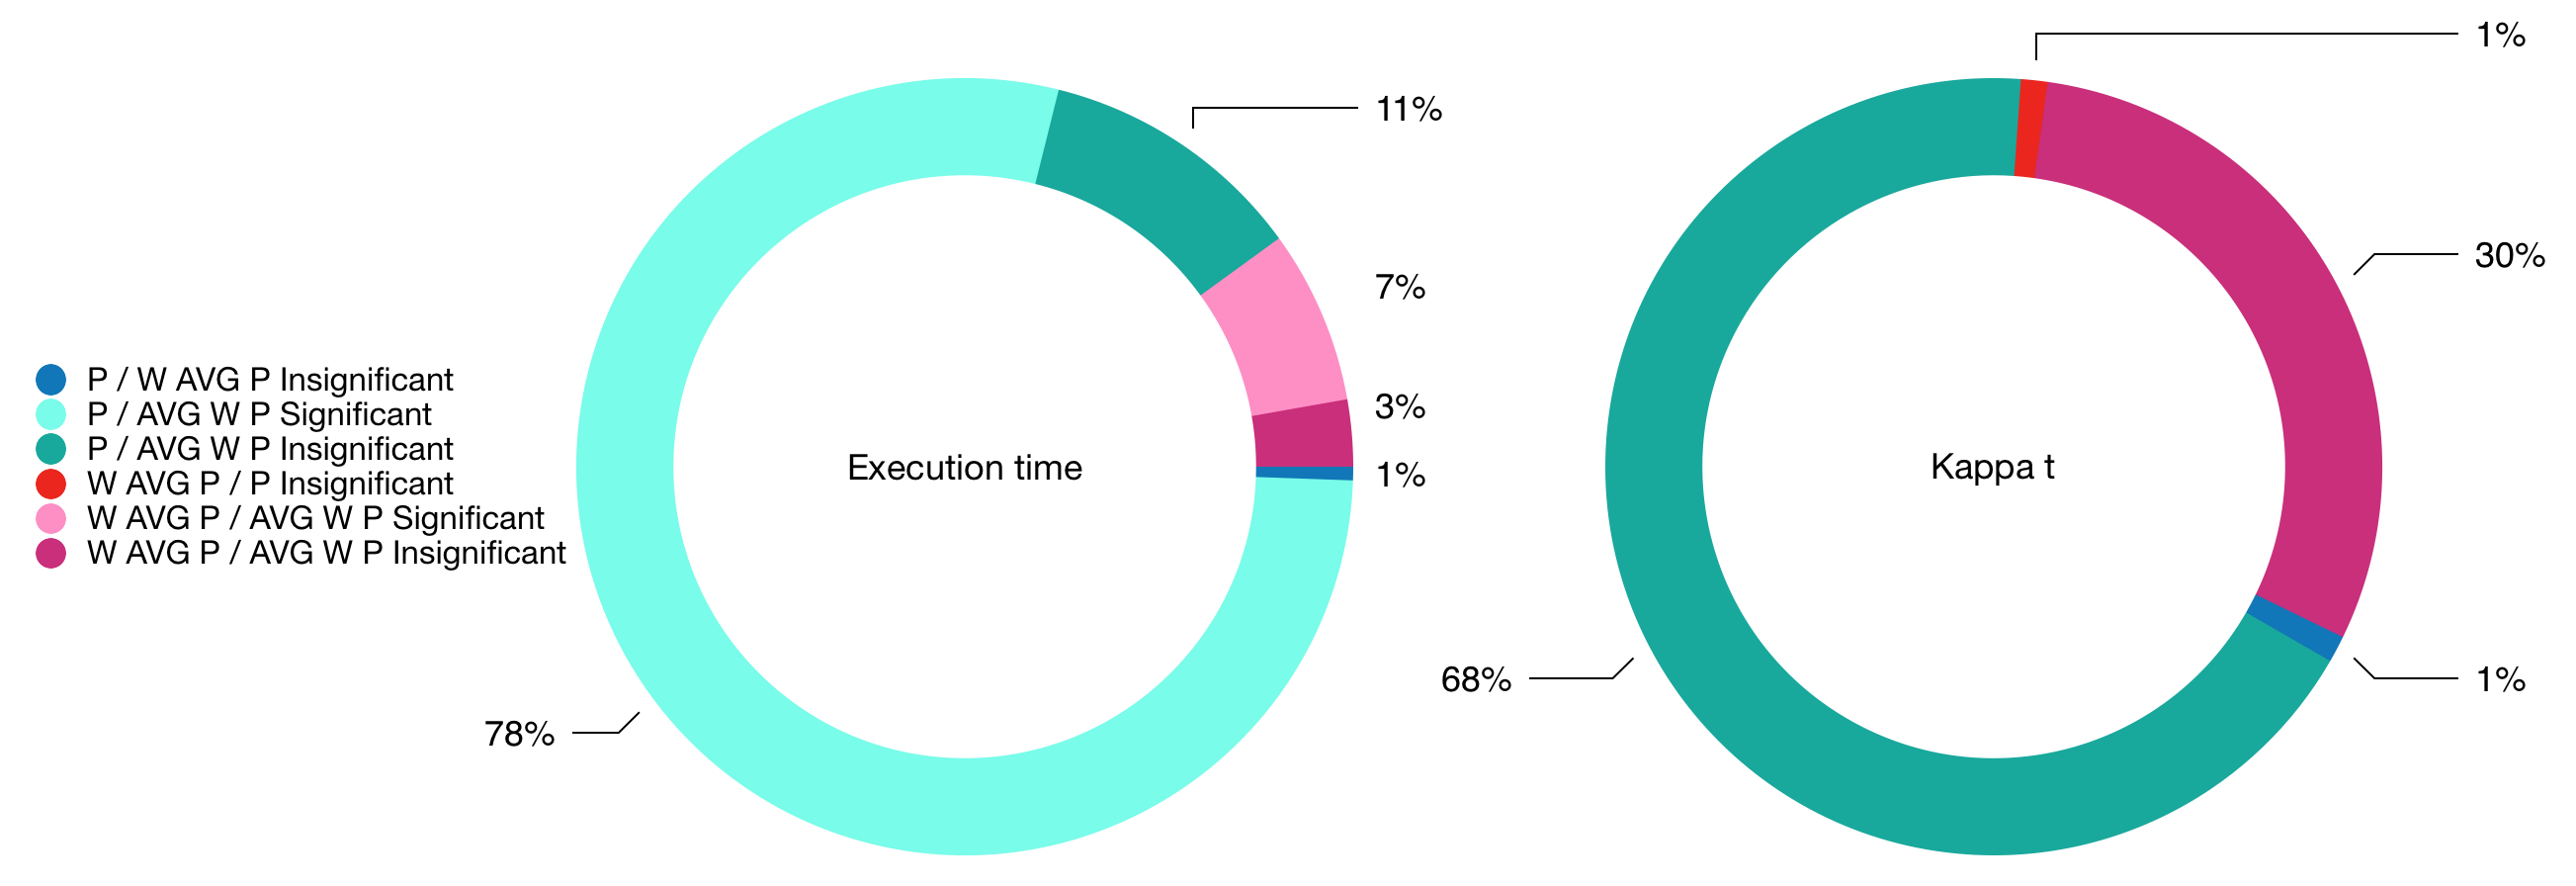
\includegraphics[width=\linewidth]{./images/chapter5/voting_type_rankings_pie}
\caption{\label{fig:voting_type_rankings_pie}Pie chart \textbf{illustrating} table \ref{table:voting_type_rankings}}
\end{figure}

\begin{sidewaysfigure}
  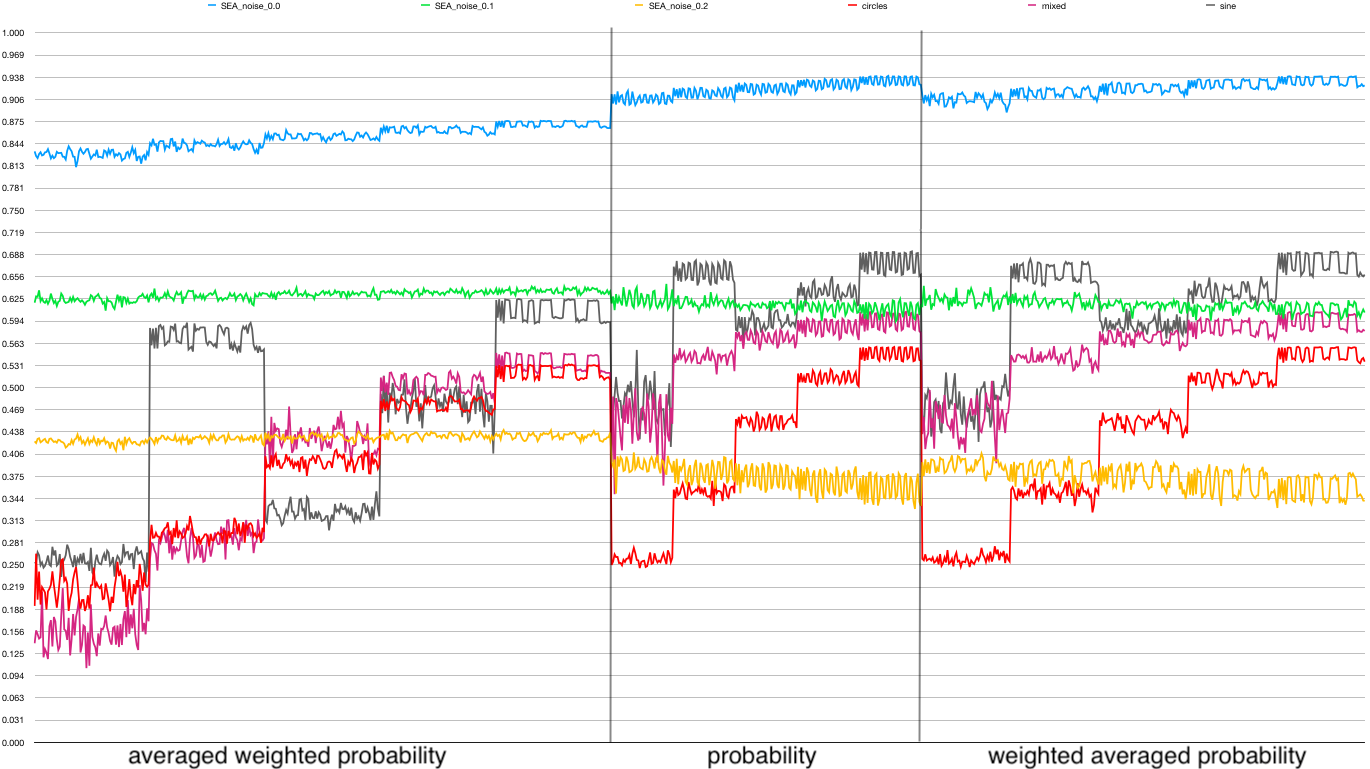
\includegraphics[width=\linewidth]{./images/chapter5/raw_voting_type}
\caption{\label{fig:order_by_voting_type}$\kappa_t$ across all parameter combinations, ordered by voting type}
\end{sidewaysfigure}

\subsection{Summary}
The above results suggest that it is preferable to use the following parameter combination to obtain higher $\kappa_t$ values: [\textit{sliding, probability, 25, $100\%$, all, 1e}].
Otherwise, to minimise the execution time, the results suggest to use [\textit{hybrid, probability, 100, $60\%$, all, 1e / 1c}].

The differences lie with the window type, the batch size, the ground truth used and partially the drift detector count. The results above indicated that using probability voting, one detector per ensemble to detect drifts, and resetting all classifiers when drifts occur would lead to better $\kappa_t$ values and a lower execution time. For the batch size, window type, and the drift detector count, it is entirely logical that choosing one value over another would change the execution time as they were, at least partially, implemented as time-saving measures.

In the following section, we will rank the parameter combinations to determine if the ones listed two paragraphs above are indeed top ranking.

\section{Comparing all parameter combinations}
In this section, we aim to rank all 1110 parameter combinations to determine which parameters perform the best, and those that perform the worst.  Recall that in the previous section, we looked at how parameter values performed individually, and this section investigates how they interact with each other. This will be done in three different configurations:
\begin{enumerate}
\item over $\kappa_t$
\item over execution time
\item over both metrics
\end{enumerate}

Due to the sheer number of parameter combinations ranked, in contrast to the few data sets used to compare them, we cannot rely on statistical significance tests. We can, however, use the algorithms in these tests to rank the combinations. We use the Nemenyi test's ranking algorithm to find the top ranking parameter combinations for our algorithm.

Parameter values are shortened to fit in tables, and their values are split by vertical lines. See table \ref{table:ranking_parameter_values_mapping} for the mapping between shortened and real parameter values. The order of the parameters in the figures are the following: [\textit{window type, voting type, ground truth, batch size, drift reset type, detector count, detector content}].

\begin{table}[]
\centering
\caption{\label{table:ranking_parameter_values_mapping}Mapping shortened parameter values with full name}
\begin{tabular}{|l|c|l|}
\hline
\textbf{Parameter} & \textbf{Value} & \textbf{Real Value} \\ \hline
\multirow{2}{*}{Window type} & s & Sliding \\ \cline{2-3} 
 & h & Hybrid \\ \hline
\multirow{4}{*}{Voting type} & aw & Averaged weighted probability \\ \cline{2-3} 
 & b & Boolean \\ \cline{2-3} 
 & p & Probability \\ \cline{2-3} 
 & wa & Weighted averaged probability \\ \hline
\multirow{4}{*}{Drift reset type} & a & All \\ \cline{2-3} 
 & b & Blind \\ \cline{2-3} 
 & n & None \\ \cline{2-3} 
 & p & Partial \\ \hline
\multirow{2}{*}{Detector count} & 1c & 1 per classifier \\ \cline{2-3} 
 & 1e & 1 for ensemble \\ \hline
\multirow{3}{*}{Detector content} & b & Boolean \\ \cline{2-3} 
 & p & Probability \\ \cline{2-3} 
 & wp & Weighted probability \\ \hline
\end{tabular}
\end{table}

\subsection{Ranking over $\kappa_t$}
% \begin{figure}
%   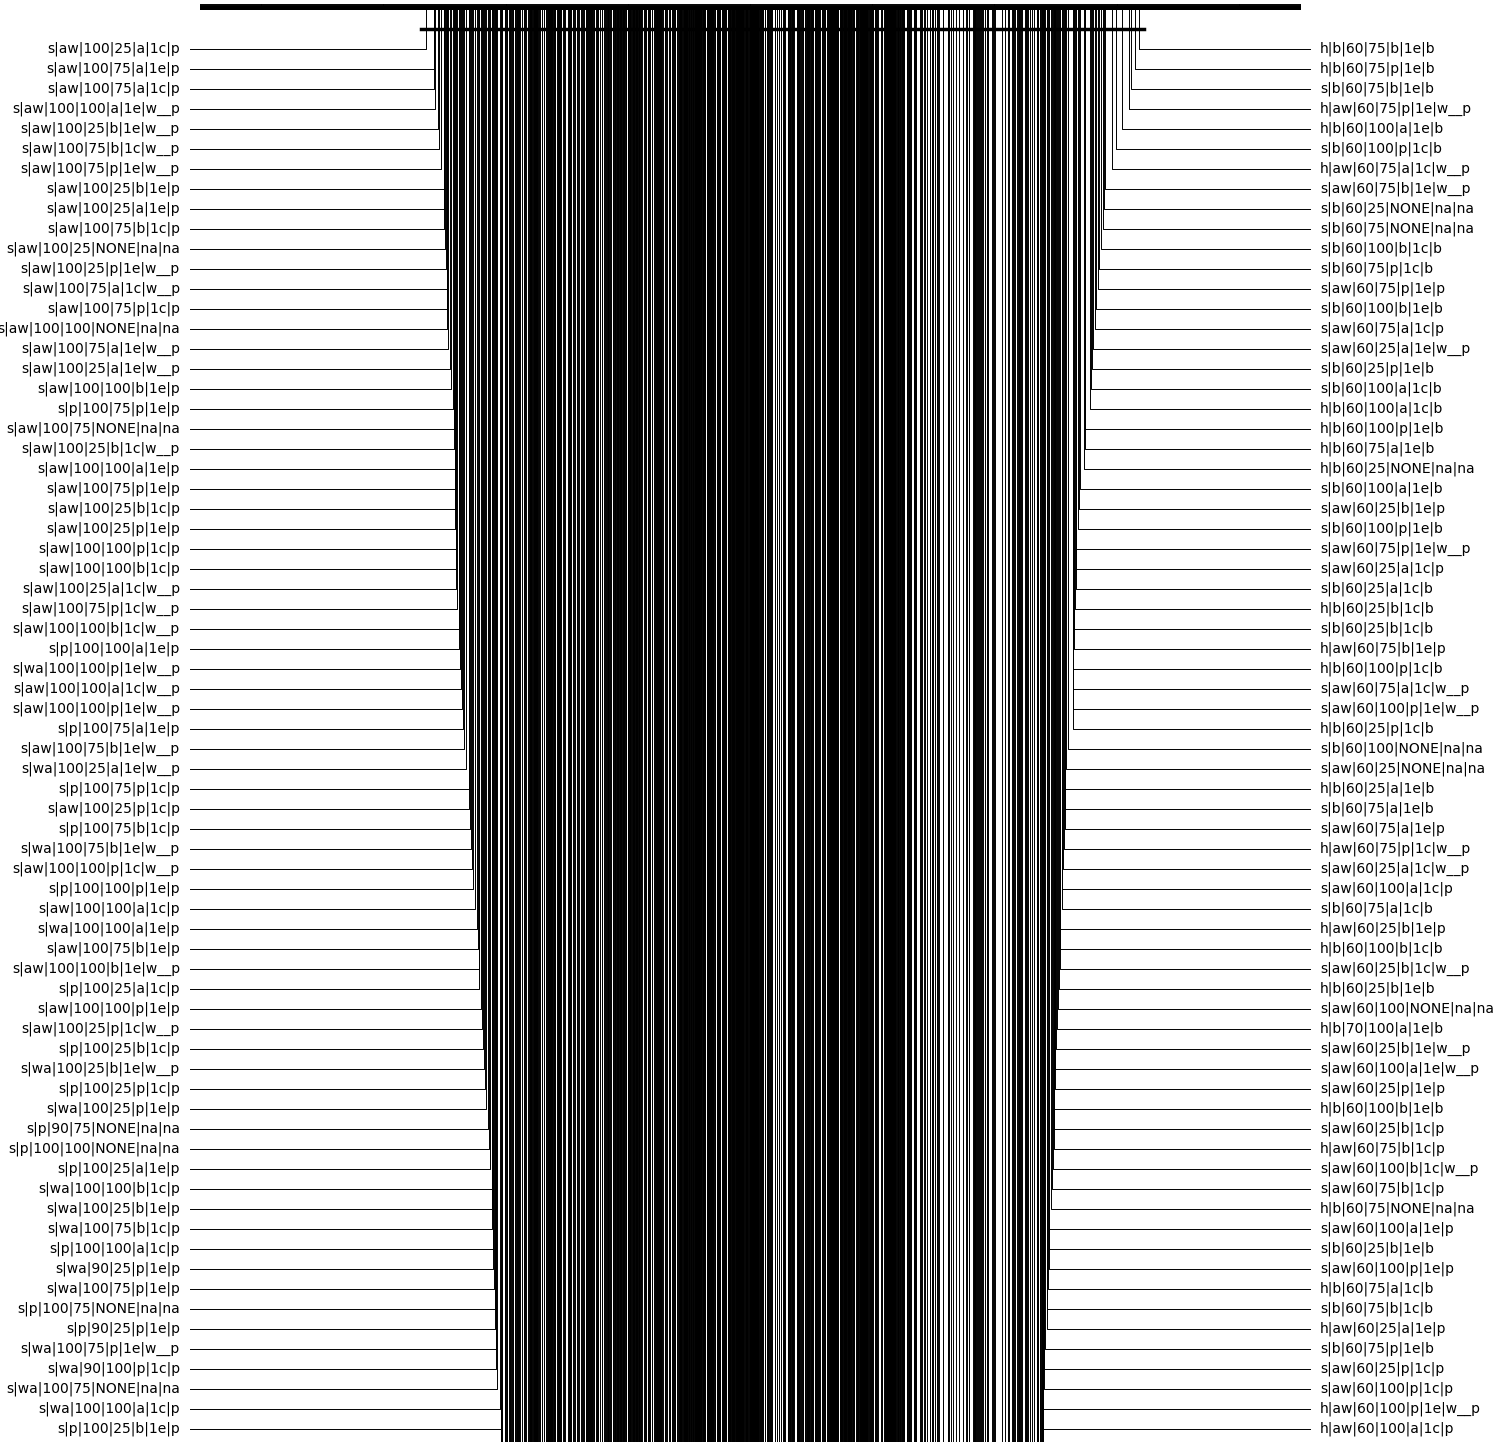
\includegraphics[width=\linewidth]{./images/chapter5/rank_kappa_cropped}
% \caption{\label{fig:rank_kappa}Ranking all parameter combinations, over $\kappa_t$}
% \end{figure}

Table \ref{table:rank_kappa_top_bottom_10}\footnote{Window type (sliding, hybrid), Voting type (averaged weighted, boolean, probability, weighted averaged), Ground Truth, Batch size, Drift reset type (all, blind, none, partial), Detector count (1 per classifier, 1 for ensemble), Detector content (boolean, probability, weighted probability)} lists the top and bottom ten ranking parameter combinations (best and worst in decreasing order, or, in other words, the combinations in the first row are the best and the worst), and table \ref{table:rank_kappa_breakdown} indicates how frequently each parameter occurred in the best 50 ranked parameter combinations for $\kappa_t$. These results suggest that parameter combinations with the following values score higher on the $\kappa_t$ metric: [\textit{sliding, *, $100\%$, 75 or 25, partial, 1c or 1e, probability}]. The asterisk is used to indicate any value for that parameter.
These findings do not precisely match up with the results found in the previous section. For example, we found that probability voting was more likely to be top ranking in the previous section, whereas we found in this section that weighted averaged or averaged weighted probability voting was more frequently in the 50 top ranked parameter combinations. The same can be said for the drift reset type parameter value.

\begin{table}[]
\centering
\caption{\label{table:rank_kappa_top_bottom_10}Top and Bottom Ten ranked parameter combinations for $\kappa_t$}
\begin{tabular}{|c|c|c|c|c|c|c||c|c|c|c|c|c|c|}
\hline
\multicolumn{7}{|c||}{\textbf{Top Ten}} & \multicolumn{7}{c|}{\textbf{Bottom Ten}} \\ \hline \hhline{=======#=======}
s & aw & 100 & 25 & a & 1c & p & h & b & 60 & 75 & b & 1e & b \\ \hline
s & aw & 100 & 75 & a & 1e & p & h & b & 60 & 75 & p & 1e & b \\ \hline
s & aw & 100 & 75 & a & 1c & p & s & b & 60 & 75 & b & 1e & b \\ \hline
s & aw & 100 & 100 & a & 1e & wp & h & aw & 60 & 75 & p & 1e & wp \\ \hline
s & aw & 100 & 25 & b & 1e & wp & h & b & 60 & 100 & a & 1e & b \\ \hline
s & aw & 100 & 75 & b & 1c & wp & s & b & 60 & 100 & p & 1c & b \\ \hline
s & aw & 100 & 75 & p & 1e & wp & h & aw & 60 & 75 & a & 1c & wp \\ \hline
s & aw & 100 & 100 & b & 1e & p & s & aw & 60 & 75 & b & 1e & wp \\ \hline
s & aw & 100 & 100 & a & 1e & p & s & b & 60 & 25 & none & none & none \\ \hline
s & aw & 100 & 100 & b & 1c & p & s & b & 60 & 75 & none & none & none \\ \hline
\end{tabular}
\end{table}

\begin{table}[]
\centering
\caption{\label{table:rank_kappa_breakdown}Breakdown of parameter value frequency in the top 50 ranked parameter combinations for $\kappa_t$}
\begin{tabular}{|l|c|c|}
\hline
\textbf{Parameter} & \textbf{Value} & \textbf{Breakdown} \\ \hline \hhline{===}
\multirow{2}{*}{Window type} & hybrid & 10\% \\ \cline{2-3} 
 & sliding & 90\% \\ \hline
\multirow{3}{*}{Voting type} & averaged weighted & 36\% \\ \cline{2-3} 
 & probability & 26\% \\ \cline{2-3} 
 & weighted averaged & 38\% \\ \hline
\multirow{2}{*}{Ground truth} & 90 & 38\% \\ \cline{2-3} 
 & 100 & 62\% \\ \hline
\multirow{3}{*}{Batch size} & 25 & 34\% \\ \cline{2-3} 
 & 75 & 38\% \\ \cline{2-3} 
 & 100 & 28\% \\ \hline
\multirow{4}{*}{Drift reset type} & all & 26\% \\ \cline{2-3} 
 & blind & 26\% \\ \cline{2-3} 
 & none & 12\% \\ \cline{2-3} 
 & partial & 36\% \\ \hline
\multirow{3}{*}{Detector count} & 1 per classifier & 42\% \\ \cline{2-3} 
 & 1 for ensemble & 46\% \\ \cline{2-3} 
 & none & 12\% \\ \hline
\multirow{3}{*}{Detector content} & probability & 68\% \\ \cline{2-3} 
 & weighted probability & 20\% \\ \cline{2-3} 
 & none & 12\% \\ \hline
\end{tabular}
\end{table}

\subsection{Ranking over execution time}
% Figure \ref{fig:rank_seconds} shows the post-hoc Nemenyi ranking results for the execution time metric. As before, the left-hand side lists the best ranking parameter combinations, and the right-hand side shows the worst performing ones. 
% We will consider the 50 top ranking parameter combinations.

% \begin{figure}
%   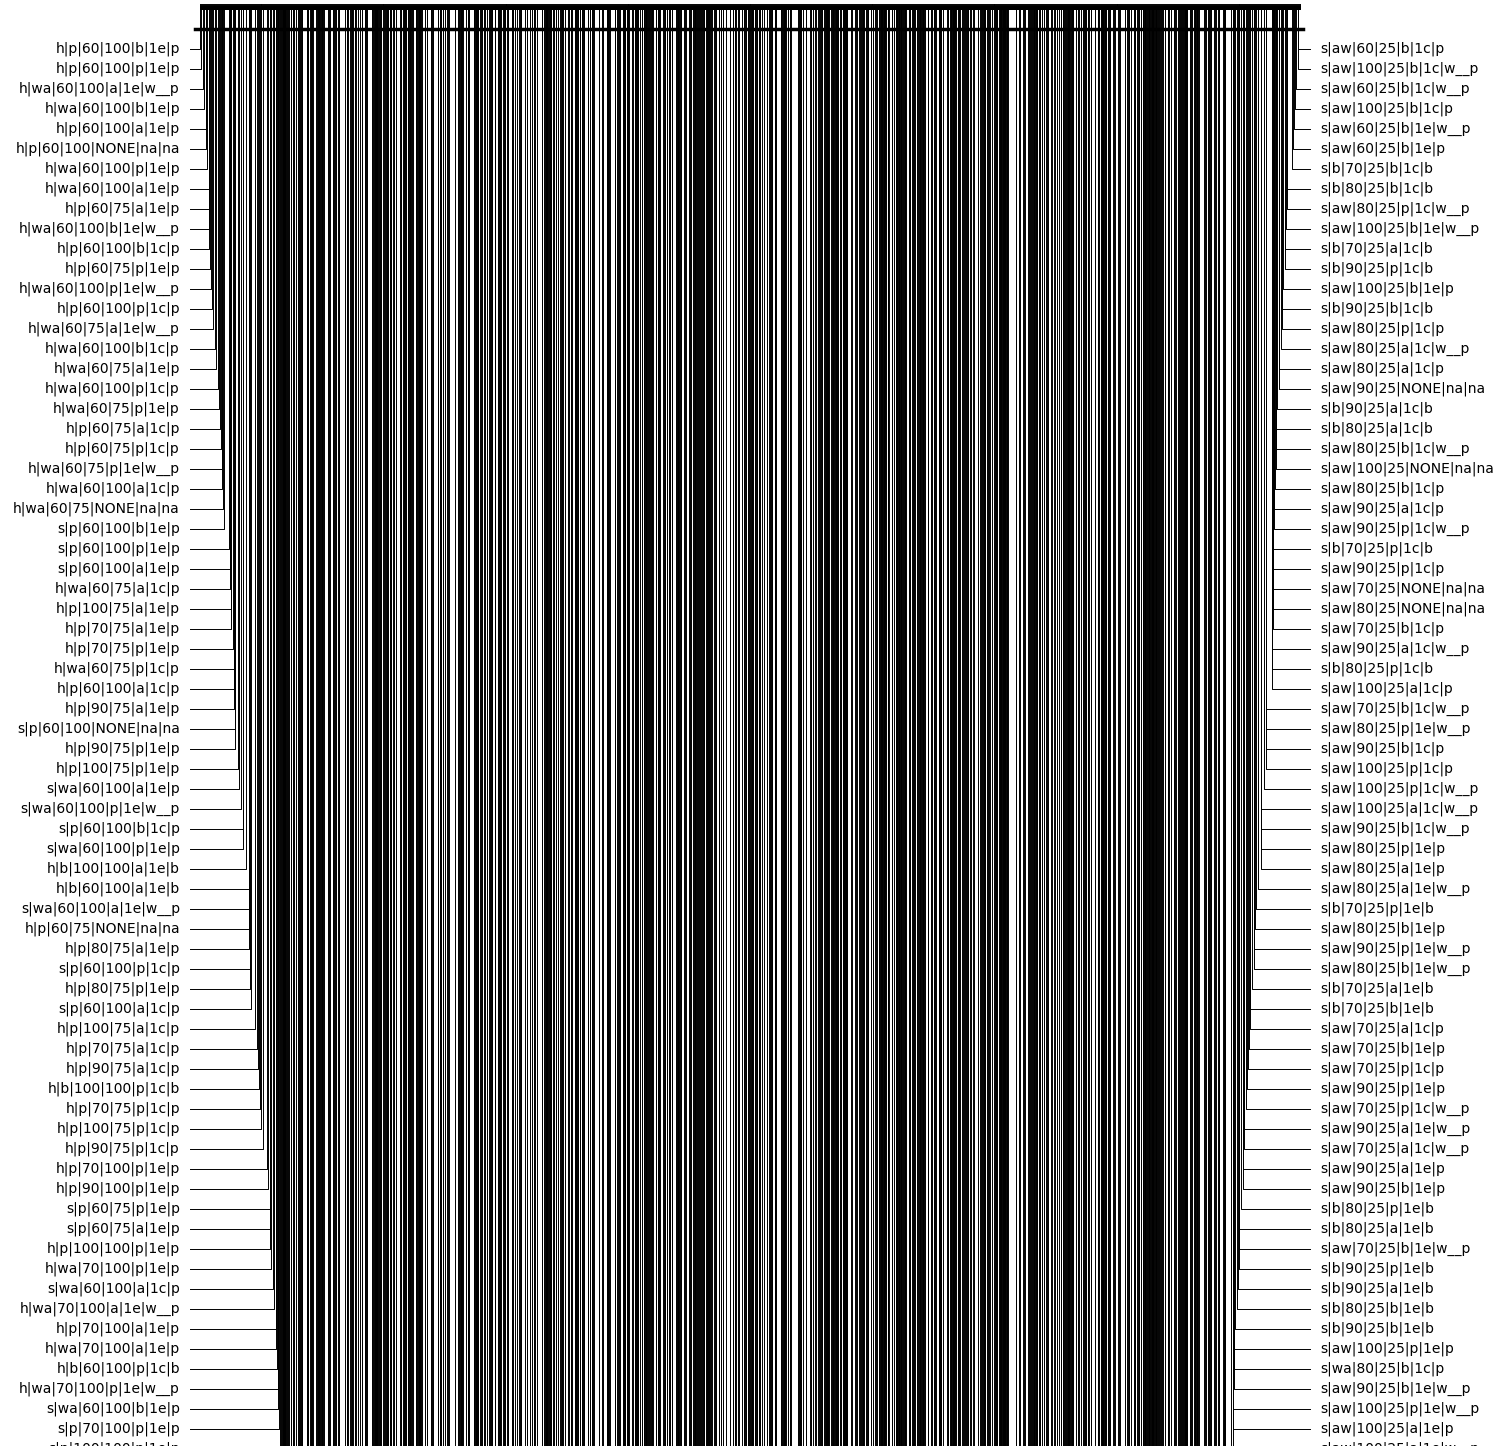
\includegraphics[width=\linewidth]{./images/chapter5/rank_seconds_cropped}
% \caption{\label{fig:rank_seconds}Ranking all parameter combinations, over execution time}
% \end{figure}

Table \ref{table:rank_seconds_top_bottom_10}\footnote{Window type (sliding, hybrid), Voting type (averaged weighted, boolean, probability, weighted averaged), Ground Truth, Batch size, Drift reset type (all, blind, none, partial), Detector count (1 per classifier, 1 for ensemble), Detector content (boolean, probability, weighted probability)} lists the top and bottom ten ranking parameter combinations, and table \ref{table:rank_seconds_breakdown} indicates how frequently each parameter occurred in the best 50 ranked parameter combinations for the execution time. These results suggest that parameter combinations with the following values have lower values for the execution time metric: [\textit{hybrid, probability, $60\%$, 100, partial, 1c or 1e, probability}]. These results almost completely match the results from the previous section, confirming our findings.

\begin{table}[]
\centering
\caption{\label{table:rank_seconds_top_bottom_10}Top and Bottom Ten ranked parameter combinations for execution time}
\begin{tabular}{|c|c|c|c|c|c|c||c|c|c|c|c|c|c|}
\hline
\multicolumn{7}{|c||}{\textbf{Top Ten}} & \multicolumn{7}{c|}{\textbf{Bottom Ten}} \\ \hline \hhline{=======#=======}
h & p & 60 & 100 & b & 1e & p & s & aw & 60 & 25 & b & 1c & p \\ \hline
h & p & 60 & 100 & p & 1e & p & s & aw & 100 & 25 & b & 1c & wp \\ \hline
h & wa & 60 & 100 & a & 1e & wp & s & aw & 60 & 25 & b & 1c & wp \\ \hline
h & wa & 60 & 100 & b & 1e & p & s & aw & 100 & 25 & b & 1c & p \\ \hline
h & p & 60 & 100 & a & 1e & p & s & aw & 60 & 25 & b & 1e & wp \\ \hline
h & p & 60 & 100 & none & none & none & s & aw & 60 & 25 & b & 1e & p \\ \hline
h & wa & 60 & 100 & p & 1e & p & s & aw & 70 & 25 & b & 1c & b \\ \hline
h & wa & 60 & 100 & a & 1e & p & s & aw & 80 & 25 & b & 1c & b \\ \hline
h & p & 60 & 75 & a & 1e & p & s & aw & 80 & 25 & p & 1c & wp \\ \hline
h & wa & 60 & 100 & b & 1e & wp & s & aw & 100 & 25 & b & 1e & wp \\ \hline
\end{tabular}
\end{table}

\begin{table}[]
\centering
\caption{\label{table:rank_seconds_breakdown}Breakdown of parameter value frequency in the top 50 ranked parameter combinations for execution time}
\begin{tabular}{|l|c|c|}
\hline
\textbf{Parameter} & \textbf{Value} & \textbf{Breakdown} \\ \hline \hhline{===}
\multirow{2}{*}{Window type} & hybrid & 78\% \\ \cline{2-3} 
 & sliding & 22\% \\ \hline
\multirow{4}{*}{Voting type} & averaged weighted & 0\% \\ \cline{2-3} 
 & boolean & 4\% \\ \cline{2-3} 
 & probability & 56\% \\ \cline{2-3} 
 & weighted averaged & 40\% \\ \hline
\multirow{5}{*}{Ground truth} & 60 & 80\% \\ \cline{2-3} 
 & 70 & 4\% \\ \cline{2-3} 
 & 80 & 4\% \\ \cline{2-3} 
 & 90 & 4\% \\ \cline{2-3} 
 & 100 & 8\% \\ \hline
\multirow{3}{*}{Batch size} & 25 & 0\% \\ \cline{2-3} 
 & 75 & 42\% \\ \cline{2-3} 
 & 100 & 58\% \\ \hline
\multirow{4}{*}{Drift reset type} & all & 42\% \\ \cline{2-3} 
 & boolean & 14\% \\ \cline{2-3} 
 & partial & 36\% \\ \cline{2-3} 
 & none & 8\% \\ \hline
\multirow{3}{*}{Detector count} & 1 per classifier & 28\% \\ \cline{2-3} 
 & 1 for ensemble & 64\% \\ \cline{2-3} 
 & none & 8\% \\ \hline
\multicolumn{1}{|c|}{\multirow{4}{*}{Detector content}} & boolean & 4\% \\ \cline{2-3} 
\multicolumn{1}{|c|}{} & probability & 74\% \\ \cline{2-3} 
\multicolumn{1}{|c|}{} & weighted probability & 14\% \\ \cline{2-3} 
\multicolumn{1}{|c|}{} & none & 8\% \\ \hline
\end{tabular}
\end{table}

\subsection{Ranking over both metrics}

By filtering the raw values from the simulations we ran, in combination with the rankings obtained in the two previous subsections, the best performing parameter combinations will be determined in this subsection.

Figure \ref{fig:rank_both_all} shows the raw values for each data set for both measured metrics. The values are ordered by an average of the ranks for $\kappa_t$ and execution time. To give more weight to the $\kappa_t$ metric in the ordering, the equation for the average is the following: 
\begin{equation}
\label{eq:rank_both}
\frac{3\times rank_{\kappa_t}+rank_{execution\ time}}{4}
\end{equation}

\begin{sidewaysfigure}
  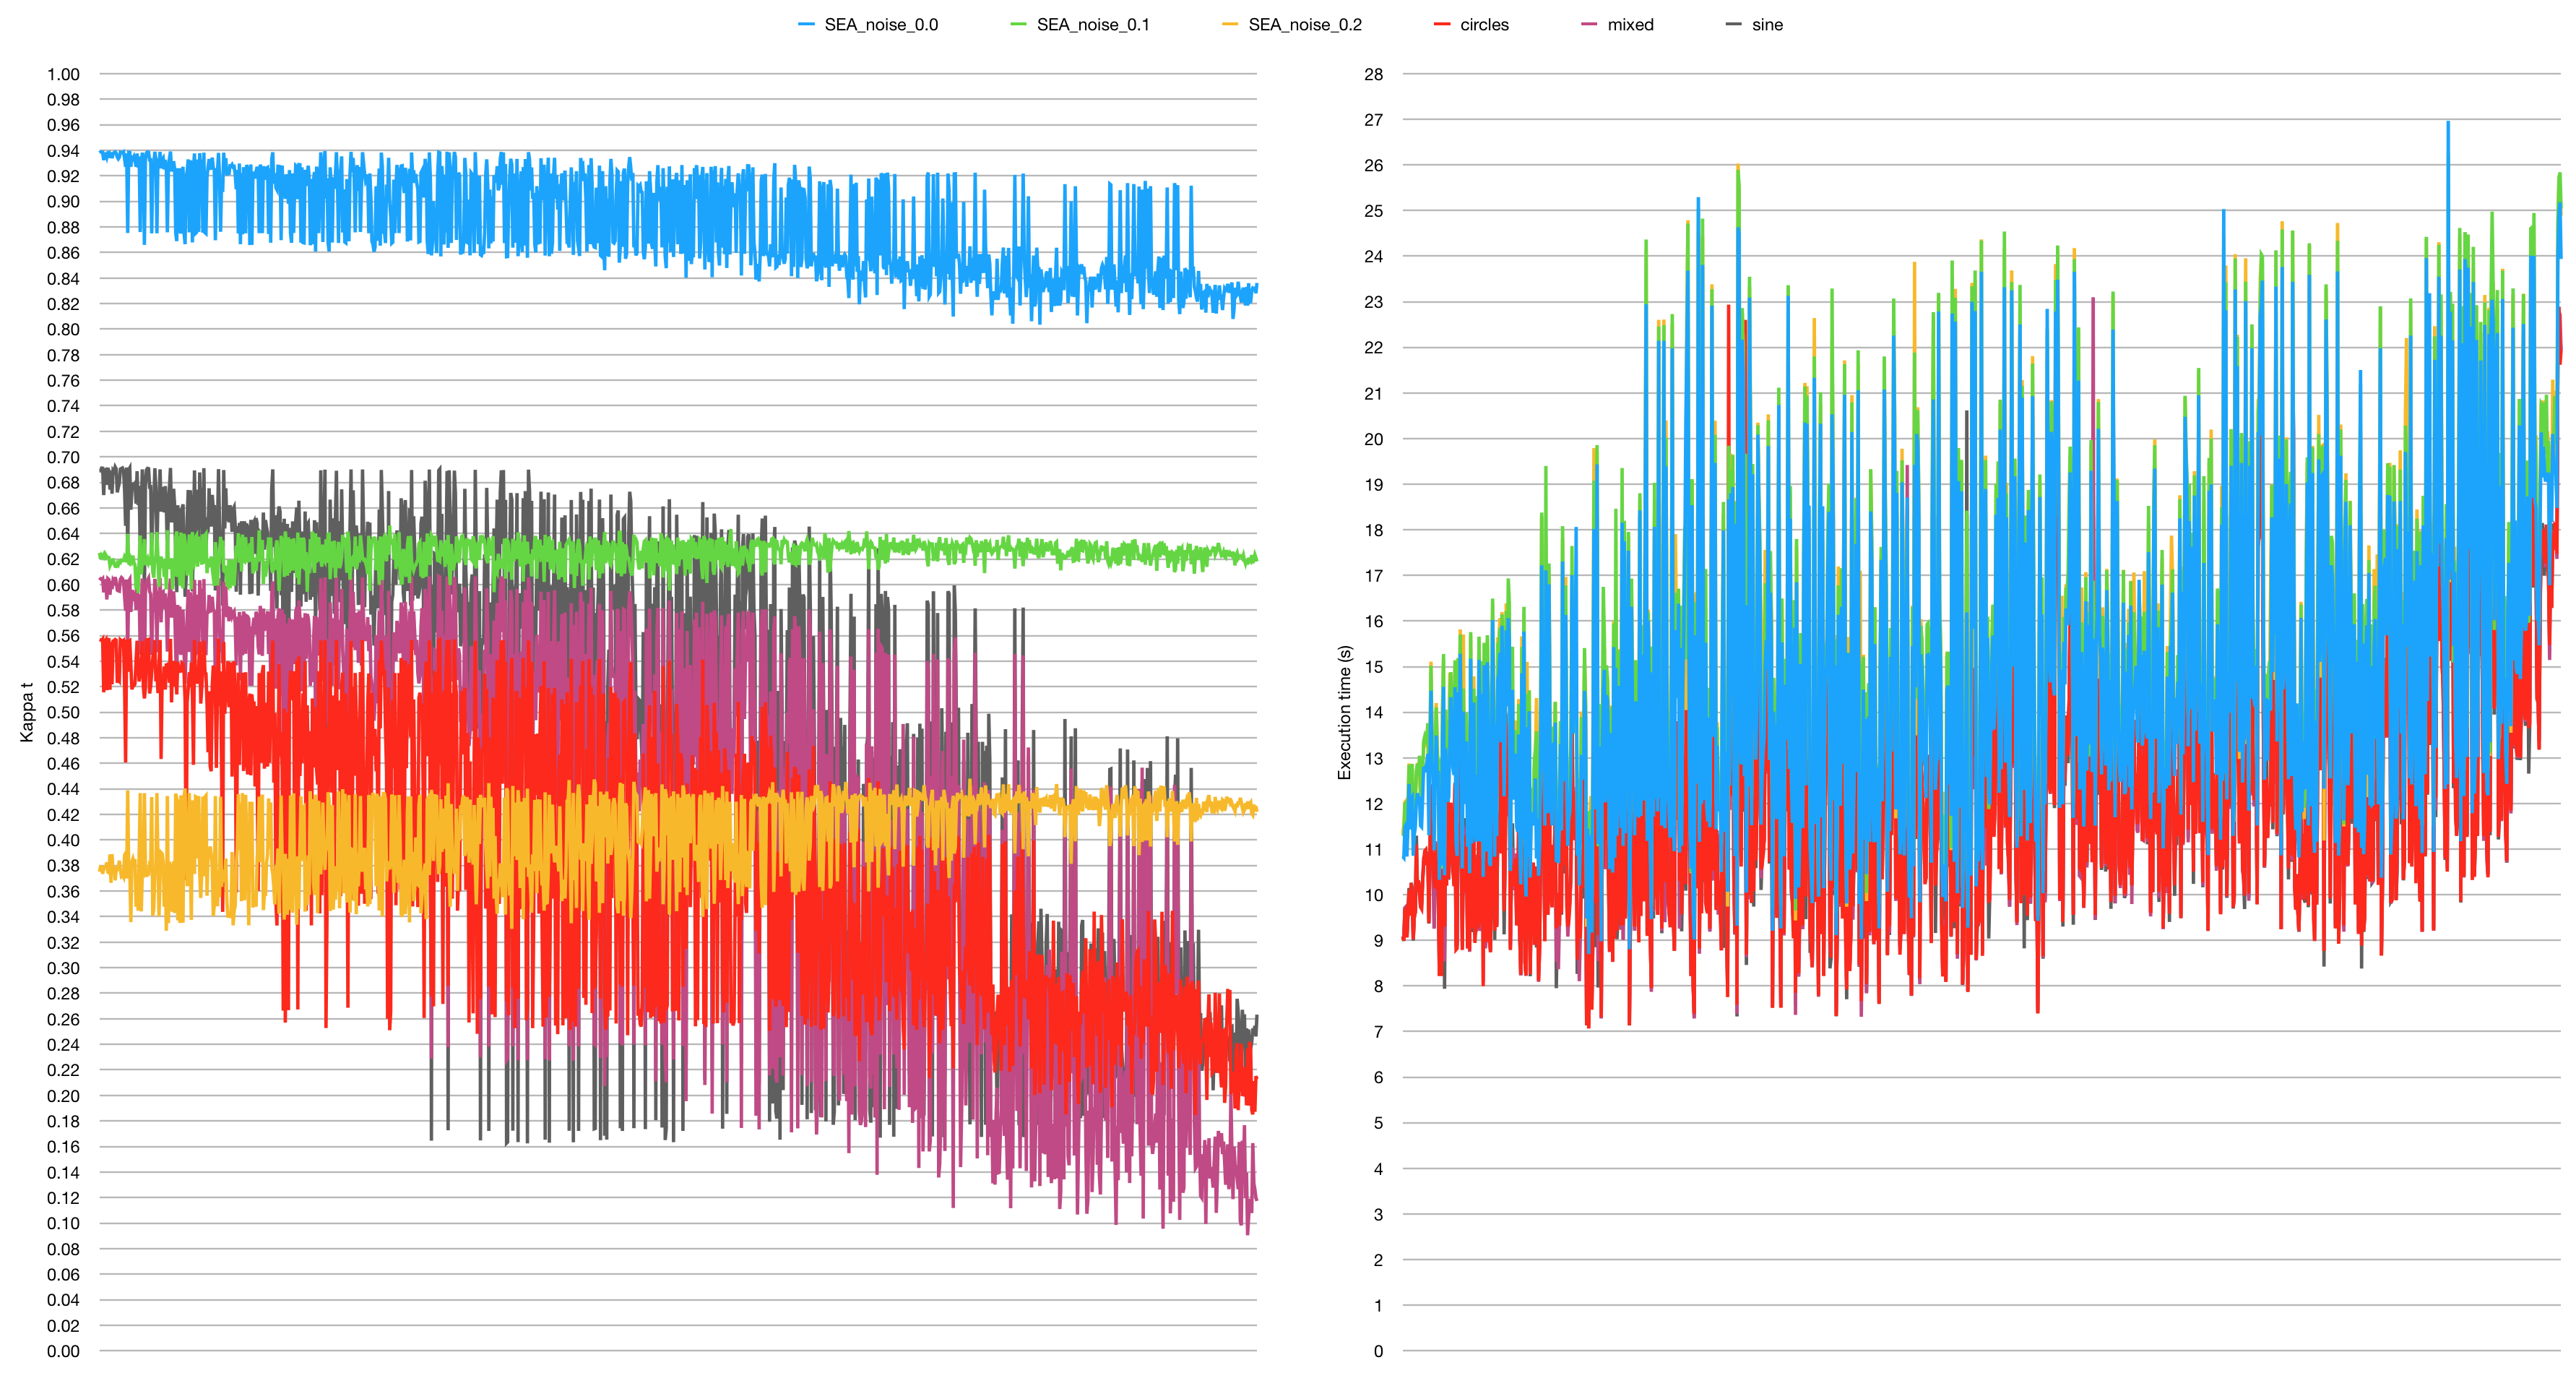
\includegraphics[width=\linewidth]{./images/chapter5/rank_both}
\caption{\label{fig:rank_both_all}Raw $\kappa_t$ and execution time values ordered by averaged ranks}
\end{sidewaysfigure}

In order to find the right balance, we started to filter out the parameter combinations with the conditions found in table \ref{table:rank_both_filter_dataset}, and then filtered out those whose averaged rank was below 340. We should note that the $\kappa_t$ ranks are in the range of $[228.8, 947.3]$ and that of the execution time in the range of $[1, 1108.2]$. Figure \ref{fig:compare_both_best} shows the remaining parameter combinations, with their raw values for both measured metrics. These filters were selected by intuition and through extensive exploration and inspection, in order to remove very high execution times as well as poor $\kappa_t$ values. We also chose to include the parameter combinations that led to the best overall $\kappa_t$ average metric, and the one with the best average execution time metric.

\begin{table}[]
\centering
\caption{\label{table:rank_both_filter_dataset}Data set filtering conditions}
\begin{tabular}{|l|c|} 
\hline
\textbf{Data set} & \textbf{Condition} \\ \hline \hhline{==}
SEA $0\%$ noise & $\le$ 11 seconds \\ \hline
circles & $\le$ 9.2 seconds \\ \hline
sine & $\le$ 9.2 seconds \\ \hline
mixed & $\le$ 9.1 seconds \\ \hline
\end{tabular}
\end{table}

\begin{sidewaysfigure}
  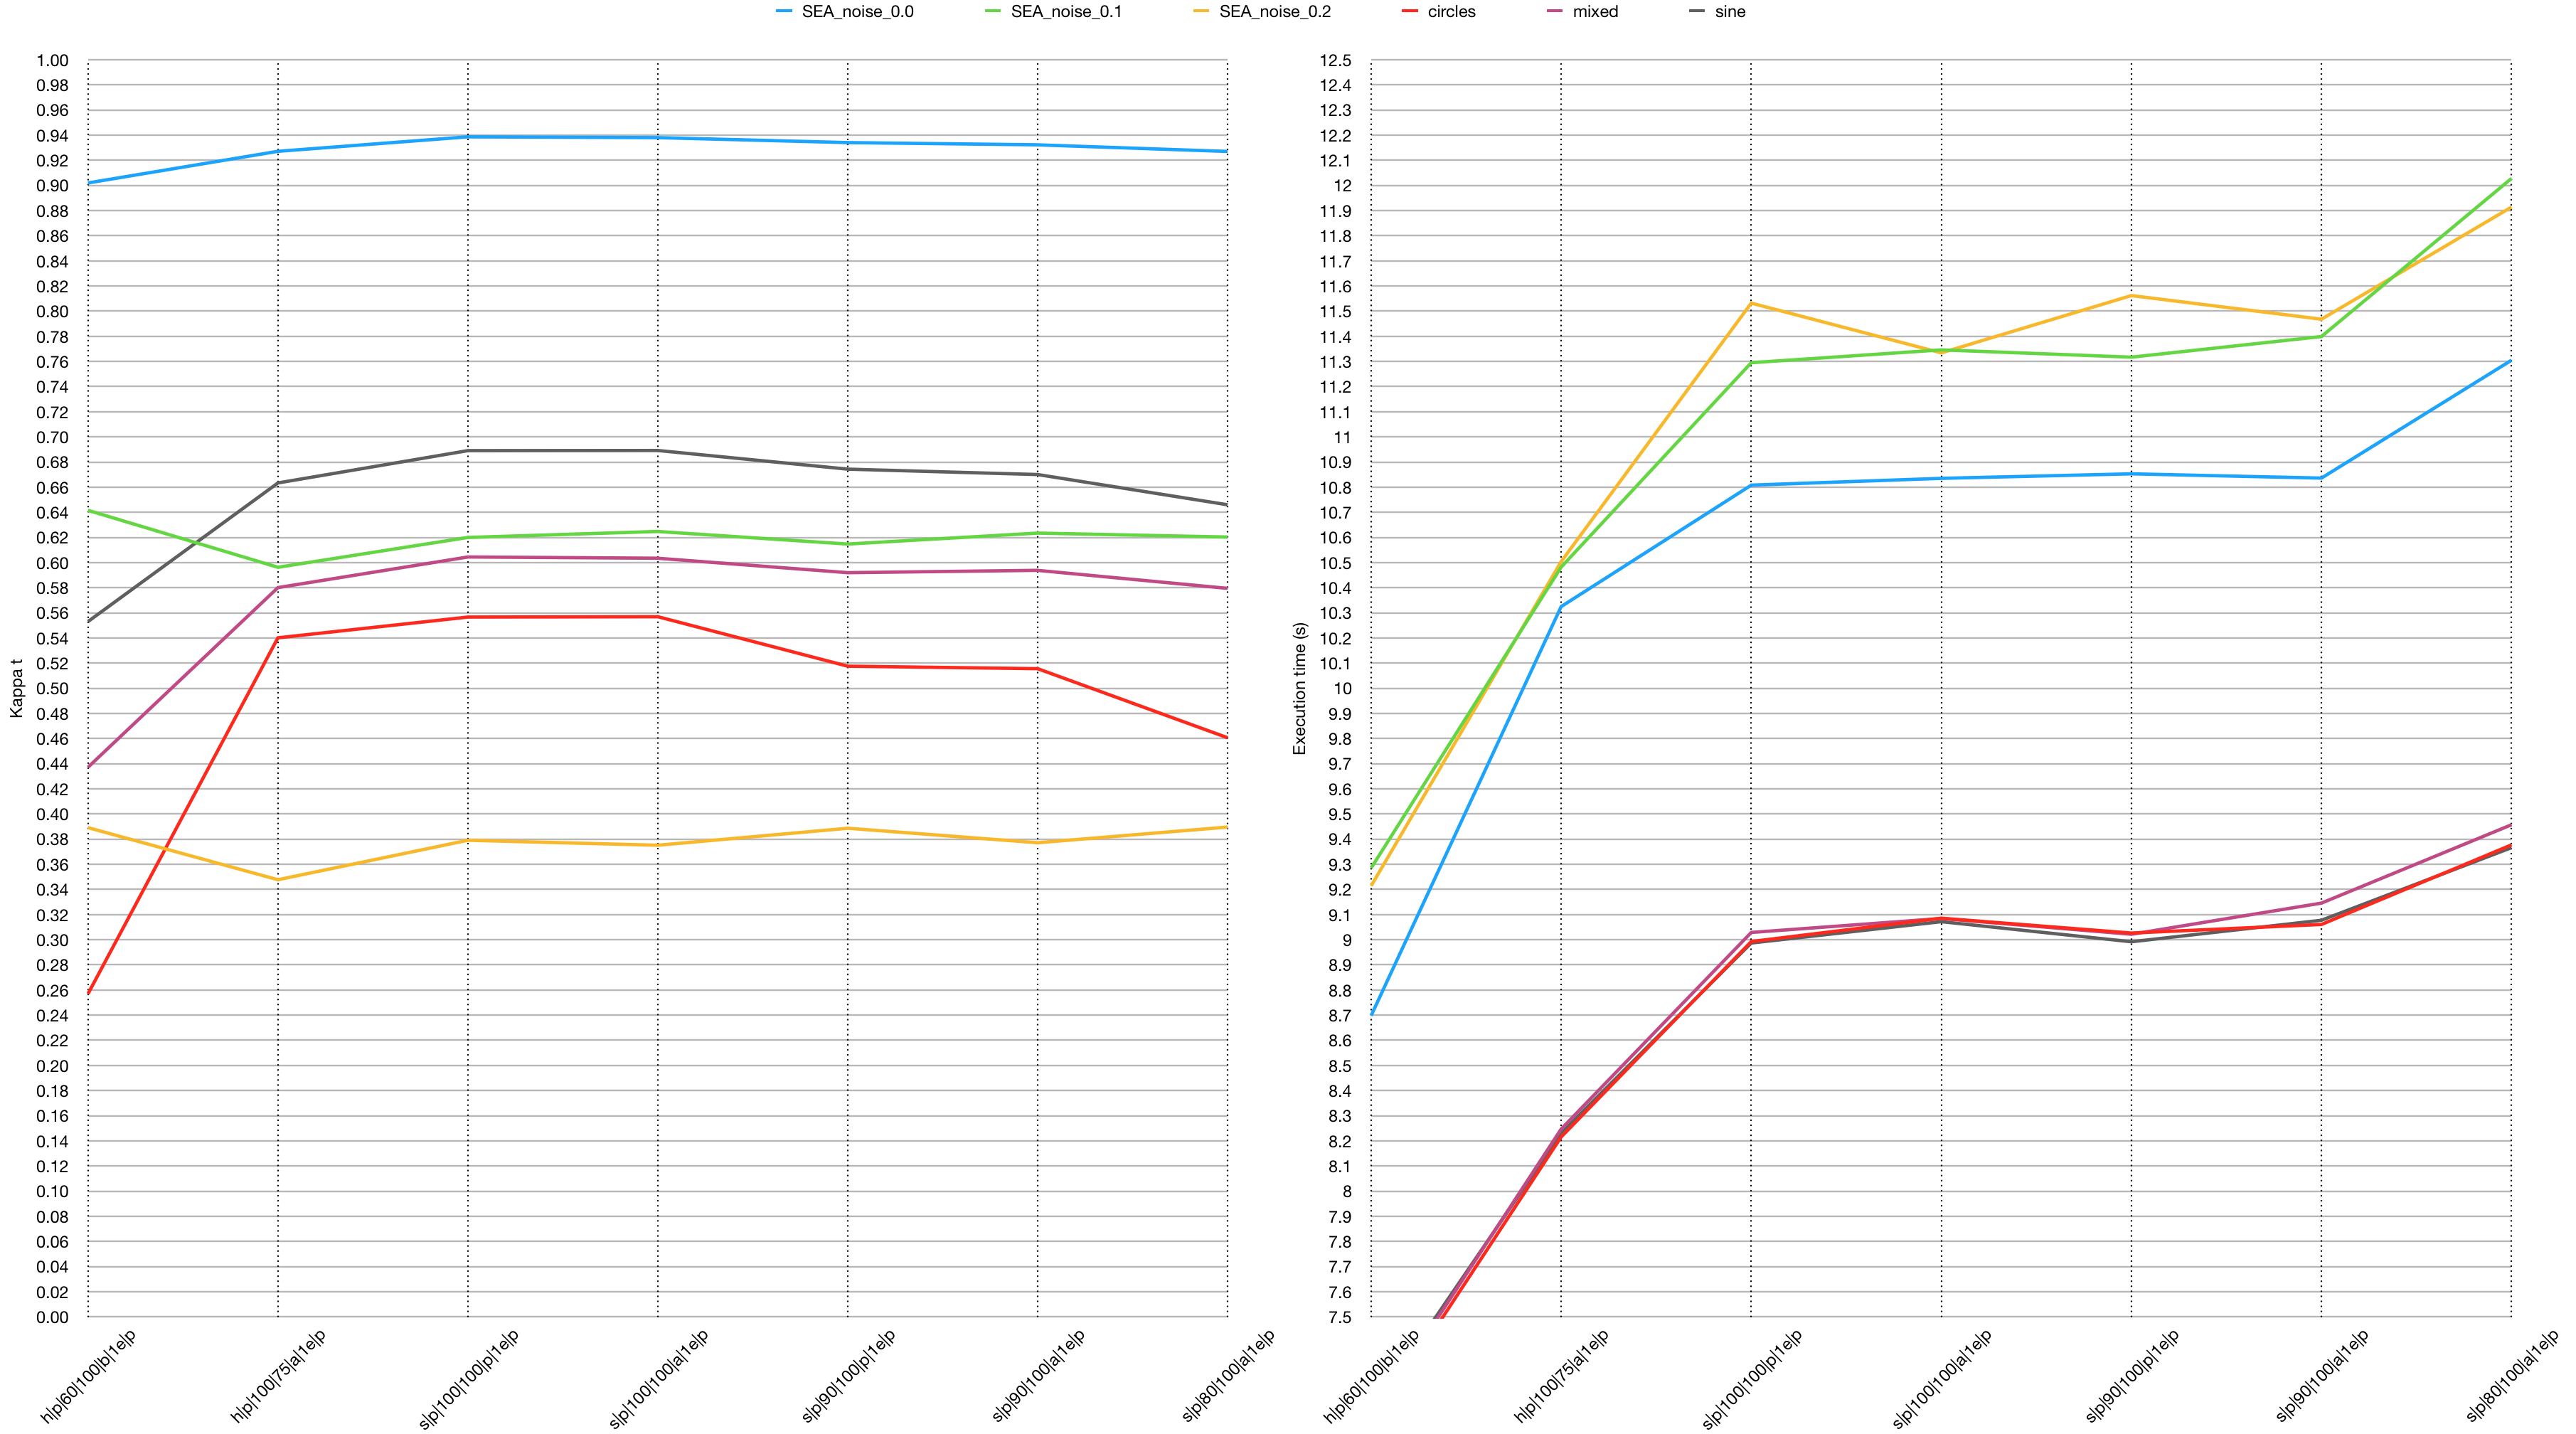
\includegraphics[width=\linewidth]{./images/chapter5/compare_both_best}
\caption{\label{fig:compare_both_best}Remaining parameter combinations and their raw metric values after filtering}
\end{sidewaysfigure}

For the best resulting predictive accuracy, [\textit{sliding window, probability voting, $100\%$ ground truth, 100 batch size, partial reset, one drift detector, probability drift content}] proved to be the best parameter combination. As for the execution time,  the following combination of parameters proved to be the best: [\textit{hybrid window, probability, $60\%$ ground truth, 100 batch size, blind reset, one drift detector, probability content}]. 

However, if we can accept a $1$ to $4\%$ reduction for $\kappa_t$ values, then significant time savings can be achieved by using [\textit{hybrid window, probability voting, $100\%$ ground truth, 75 batch size, reset all, one drift detector, probability content}]. Indeed, we can reduce execution time by up to $9.5\%$.

\subsection{Effects of training with less labelled data}
\begin{sidewaysfigure}
  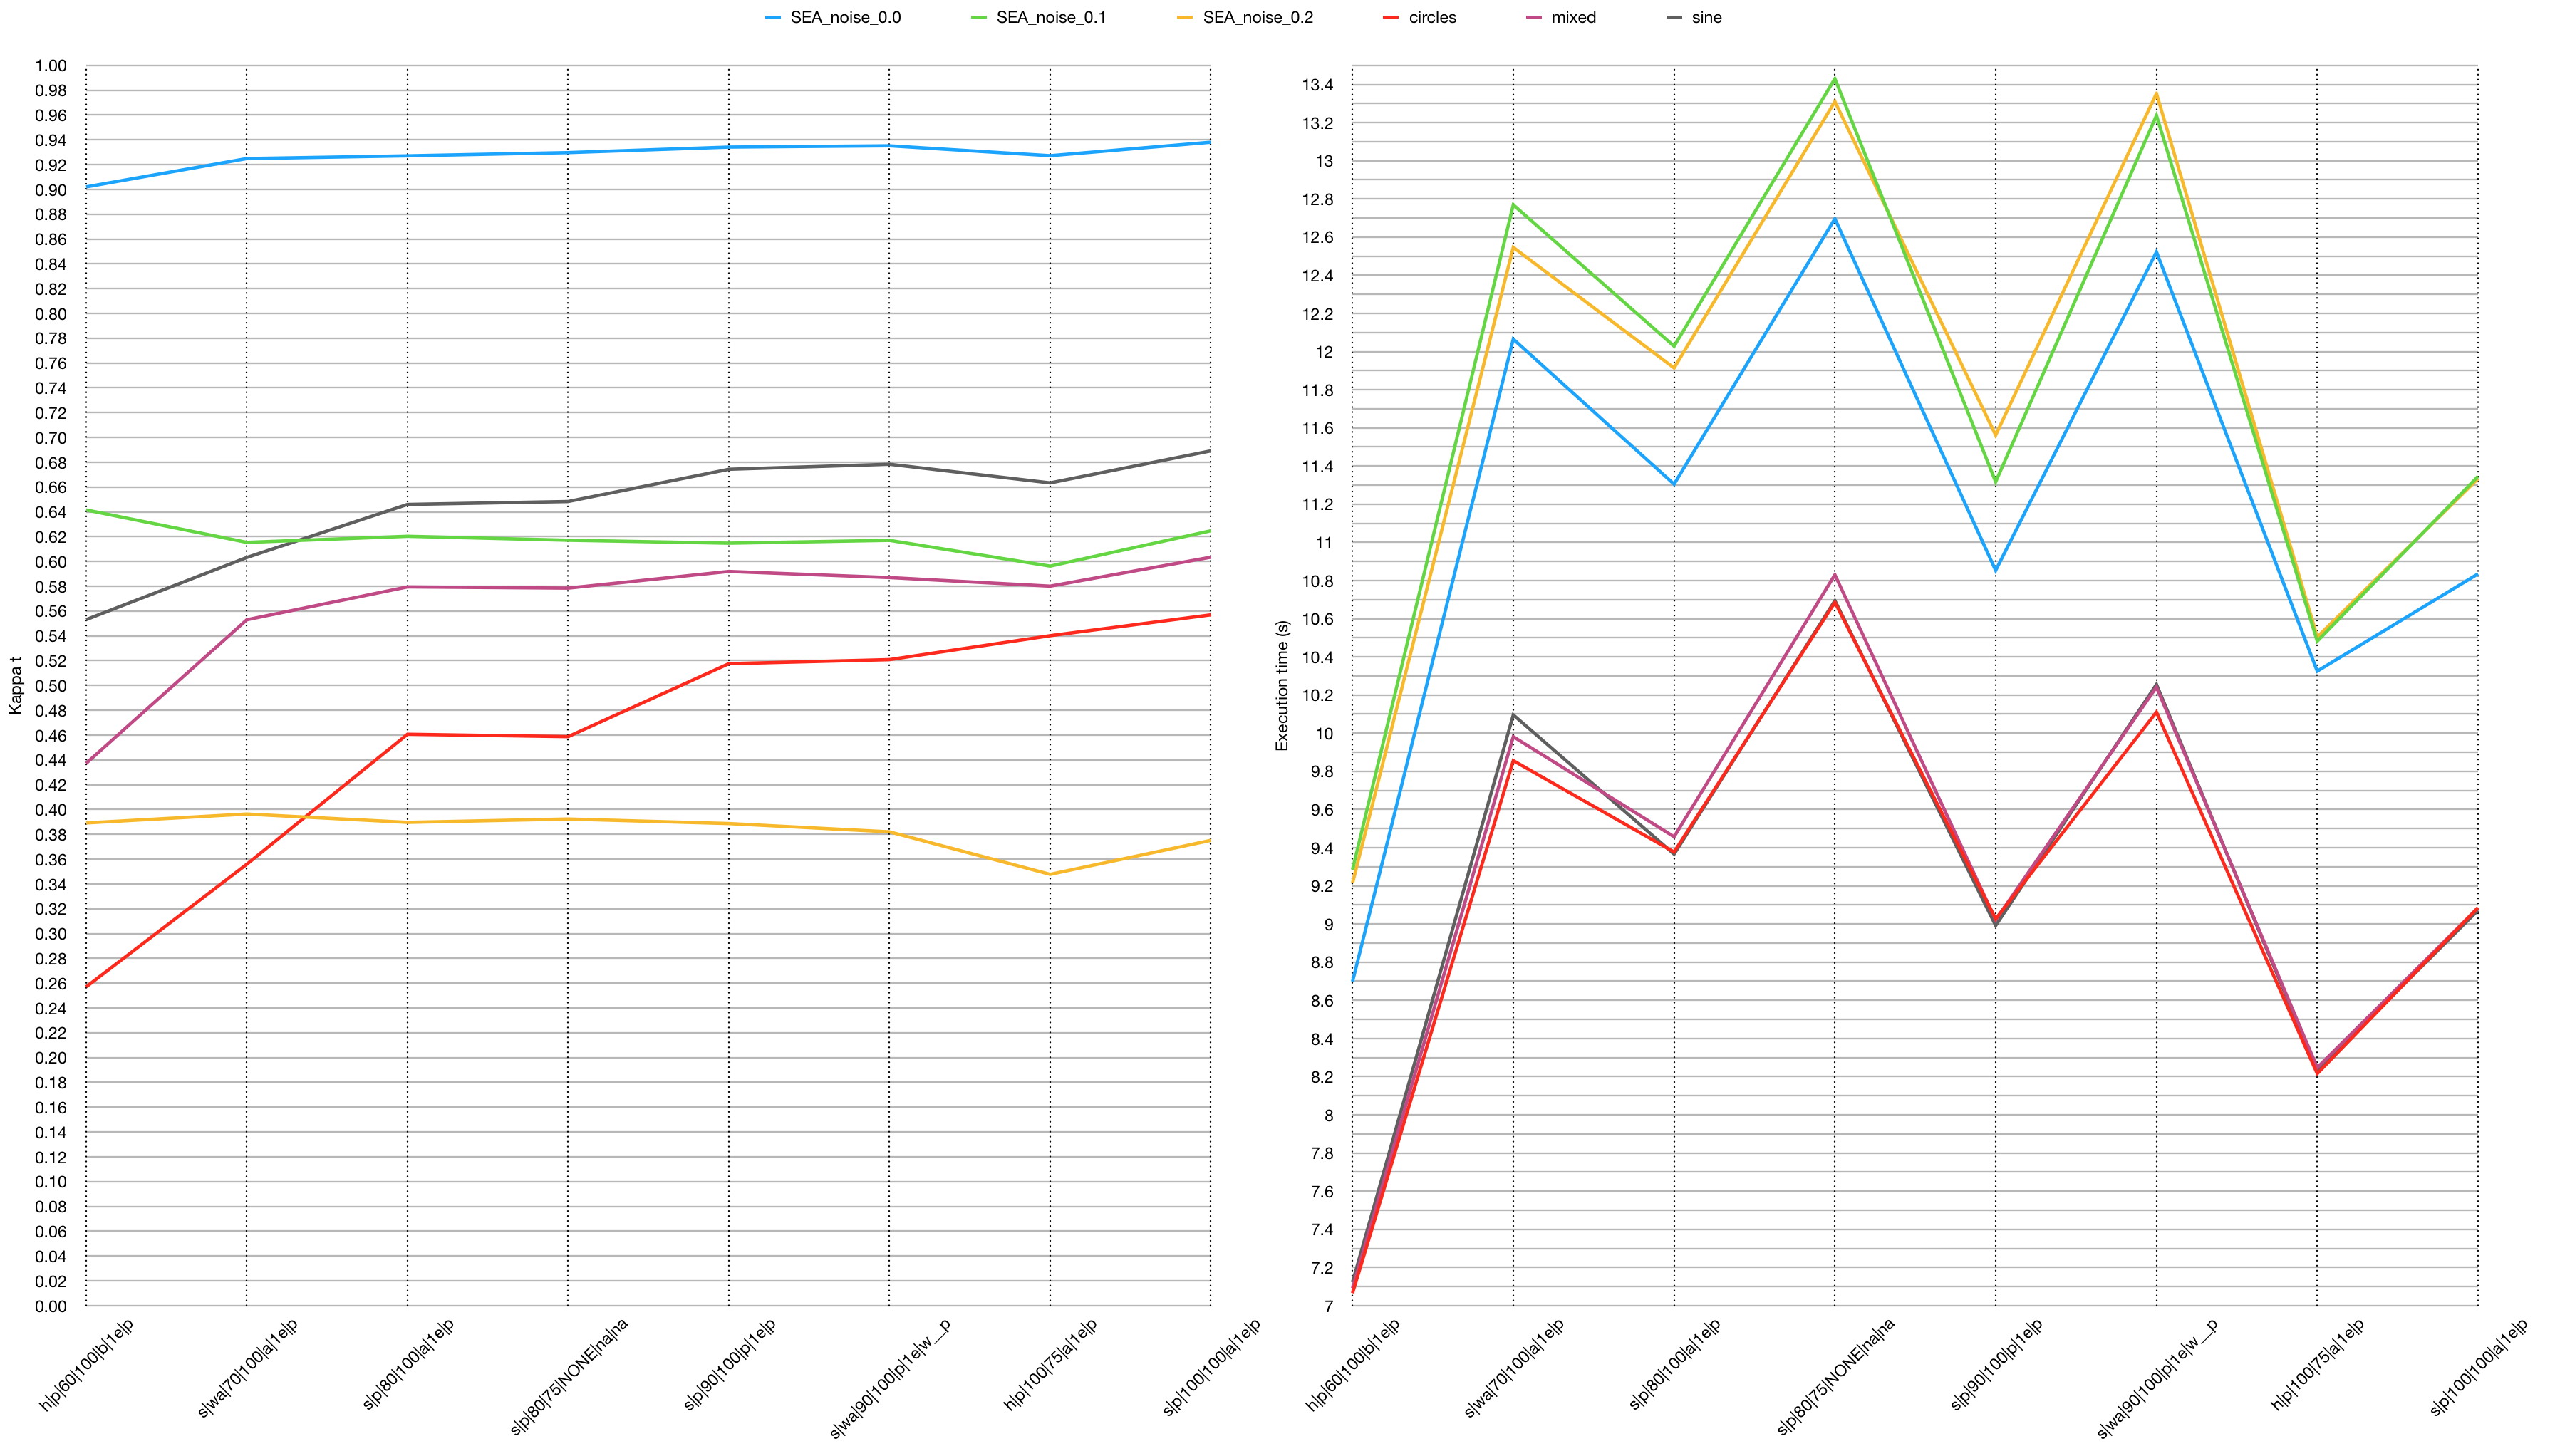
\includegraphics[width=\linewidth]{./images/chapter5/ground_truth_both}
\caption{\label{fig:ground_truth_drop}$\kappa_t$ and execution times for parameter combinations using varying amounts of ground truth}
\end{sidewaysfigure}

As stated in section \ref{section:vc_reduce_gt}, we aim to determine the percentage of labelled data used \textbf{at} which our voting ensemble's $\kappa_t$ metric declines and by how much. Figure \ref{fig:ground_truth_drop} shows the predictive performance and execution times for parameter combinations with varying amounts of ground truth (ten percent increments starting at 60\%). The combinations were selected by inspection after having been ranked with the averaging equation (\ref{eq:rank_both}) shown above. Table \ref{table:ground_truth_Acc_kappa} lists the global predictive accuracy and the $\kappa_t$ values for each data set for some of the parameter values used in figure \ref{fig:ground_truth_drop}. This table indicates that the global predictive accuracy of our ensemble is not significantly reduced by training with less ground truth. However, the predictive performance of the ensemble, as measured by $\kappa_t$, differs between 20\% and 54\% when examining $\kappa_t$ when using 60\% and 100\% of ground truth. The $\kappa_t$ results indicate that as the ensemble trains with less labelled data, it performs more similarly to a baseline no-change classifier (refer to section \ref{section:kappa_t}).

\begin{table}[]
  \centering
  \caption{Accuracy (\%) and $\kappa_t$ when training with varying percentages of labelled data for the parameter combinations in figure \ref{fig:ground_truth_drop}.
  \label{table:ground_truth_Acc_kappa}}
  \begin{tabular}{|c||c|c|c|c|c|c|c|c|c|c|c|c|}
  \hline
   & \multicolumn{2}{c|}{\textbf{CIRCLES}} & \multicolumn{2}{c|}{\textbf{MIXED}} & \multicolumn{2}{c|}{\textbf{SINE1}} & \multicolumn{2}{c|}{\textbf{SEA 0\%}} & \multicolumn{2}{c|}{\textbf{SEA 10\%}} & \multicolumn{2}{c|}{\textbf{SEA 20\%}} \\ \cline{2-13} 
\multirow{-2}{*}{\textbf{GT}} & \multicolumn{1}{c|}{\textbf{Acc}} & \multicolumn{1}{c|}{\textbf{$\kappa_t$}} & \multicolumn{1}{c|}{\textbf{Acc}} & \multicolumn{1}{c|}{\textbf{$\kappa_t$}} & \multicolumn{1}{c|}{\textbf{Acc}} & \multicolumn{1}{c|}{\textbf{$\kappa_t$}} & \multicolumn{1}{c|}{\textbf{Acc}} & \multicolumn{1}{c|}{\textbf{$\kappa_t$}} & \multicolumn{1}{c|}{\textbf{Acc}} & \multicolumn{1}{c|}{\textbf{$\kappa_t$}} & \multicolumn{1}{c|}{\textbf{Acc}} & \multicolumn{1}{c|}{\textbf{$\kappa_t$}} \\ \hhline{=============}
  \textbf{100} & {\color[HTML]{656565} 78} & 0.56 & {\color[HTML]{656565} 80} & 0.60 & {\color[HTML]{656565} 84} & 0.69 & {\color[HTML]{656565} 97} & 0.94 & {\color[HTML]{656565} 82} & 0.62 & {\color[HTML]{656565} 70} & 0.38 \\ \hline
  \textbf{90} & {\color[HTML]{656565} 76} & 0.52 & {\color[HTML]{656565} 79} & 0.59 & {\color[HTML]{656565} 84} & 0.68 & {\color[HTML]{656565} 97} & 0.94 & {\color[HTML]{656565} 82} & 0.62 & {\color[HTML]{656565} 70} & 0.38 \\ \hline
  \textbf{80} & {\color[HTML]{656565} 73} & 0.46 & {\color[HTML]{656565} 79} & 0.58 & {\color[HTML]{656565} 82} & 0.65 & {\color[HTML]{656565} 96} & 0.93 & {\color[HTML]{656565} 82} & 0.62 & {\color[HTML]{656565} 70} & 0.39 \\ \hline
  \textbf{70} & {\color[HTML]{656565} 68} & 0.36 & {\color[HTML]{656565} 77} & 0.55 & {\color[HTML]{656565} 80} & 0.60 & {\color[HTML]{656565} 96} & 0.92 & {\color[HTML]{656565} 82} & 0.62 & {\color[HTML]{656565} 71} & 0.40 \\ \hline
  \textbf{60} & {\color[HTML]{656565} 63} & 0.26 & {\color[HTML]{656565} 72} & 0.44 & {\color[HTML]{656565} 77} & 0.55 & {\color[HTML]{656565} 95} & 0.90 & {\color[HTML]{656565} 83} & 0.64 & {\color[HTML]{656565} 70} & 0.39 \\ \hline
  \end{tabular}
  \end{table}

One finding that we find particularly odd is that as the use of ground truth diminishes, the predictive accuracy increases for the SEA generated data sets with noise. We are led to believe that for increasing levels of noise in a data set, reducing the ground truth used (to an extent) to train a model increases its predictive performance. Further research, outside the scope of this thesis, is needed to ascertain the veracity of this finding. We posit that data generated by SEA is much easier to model than data from CIRCLES, for example, therefore requiring much less labelled data to model.

From figure \ref{fig:ground_truth_drop} and table \ref{table:ground_truth_Acc_kappa}, we find that our ensemble does not suffer a drastic reduction in its global predictive accuracy when training with only 60\% ground truth (in other words, training with 40\% less labelled data). However, the $\kappa_t$ statistic indicates that training our ensemble using non-selective self-training on a data set containing less than 70\% labelled data results in a predictive performance that is not drastically better than a no-change classifier (for the most part, as results for SEA and the other data sets highly differ). Additionally, we can see that the CIRCLES data set is harder to model with access to less labelled data, which is perfectly logical given what the class label represents. Indeed, very specific data instances are required to model the class well, given that it represents whether or not a data instance resides within the radius of a predefined circle.

It is clear that the reduction in $\kappa_t$ is dependant on both the data set being modelled as well as how much of that data set is labelled. Overall, we find that training our ensemble with a data set that is 80\% or 90\% labelled leads to a good predictive accuracy (as measured by $\kappa_t$).

\section{Comparing to the State of the Art}

Now that we have determined which parameter combinations worked particularly well, we can compare them to the State of the Art.

As previously mentioned, the algorithms which we will be comparing our voting ensemble to will be mainly the Leveraging Bagging algorithm. As we explained in the chapter \ref{chapter:background_work}, the Leveraging Bagging (section \ref{section:leveraging-bagging}) will be comprised of 10 Hoeffding Tree (section \ref{section:vfdt}) estimators, each with its own ADWIN drift detector. We will also be using a regular Hoeffding Tree using the default parameters without any drift detector. Finally, we will also include a no-change and a majority class classifier in our comparison.

\subsection{Choosing a window size for State of the Art algorithms}

\begin{sidewaysfigure}
  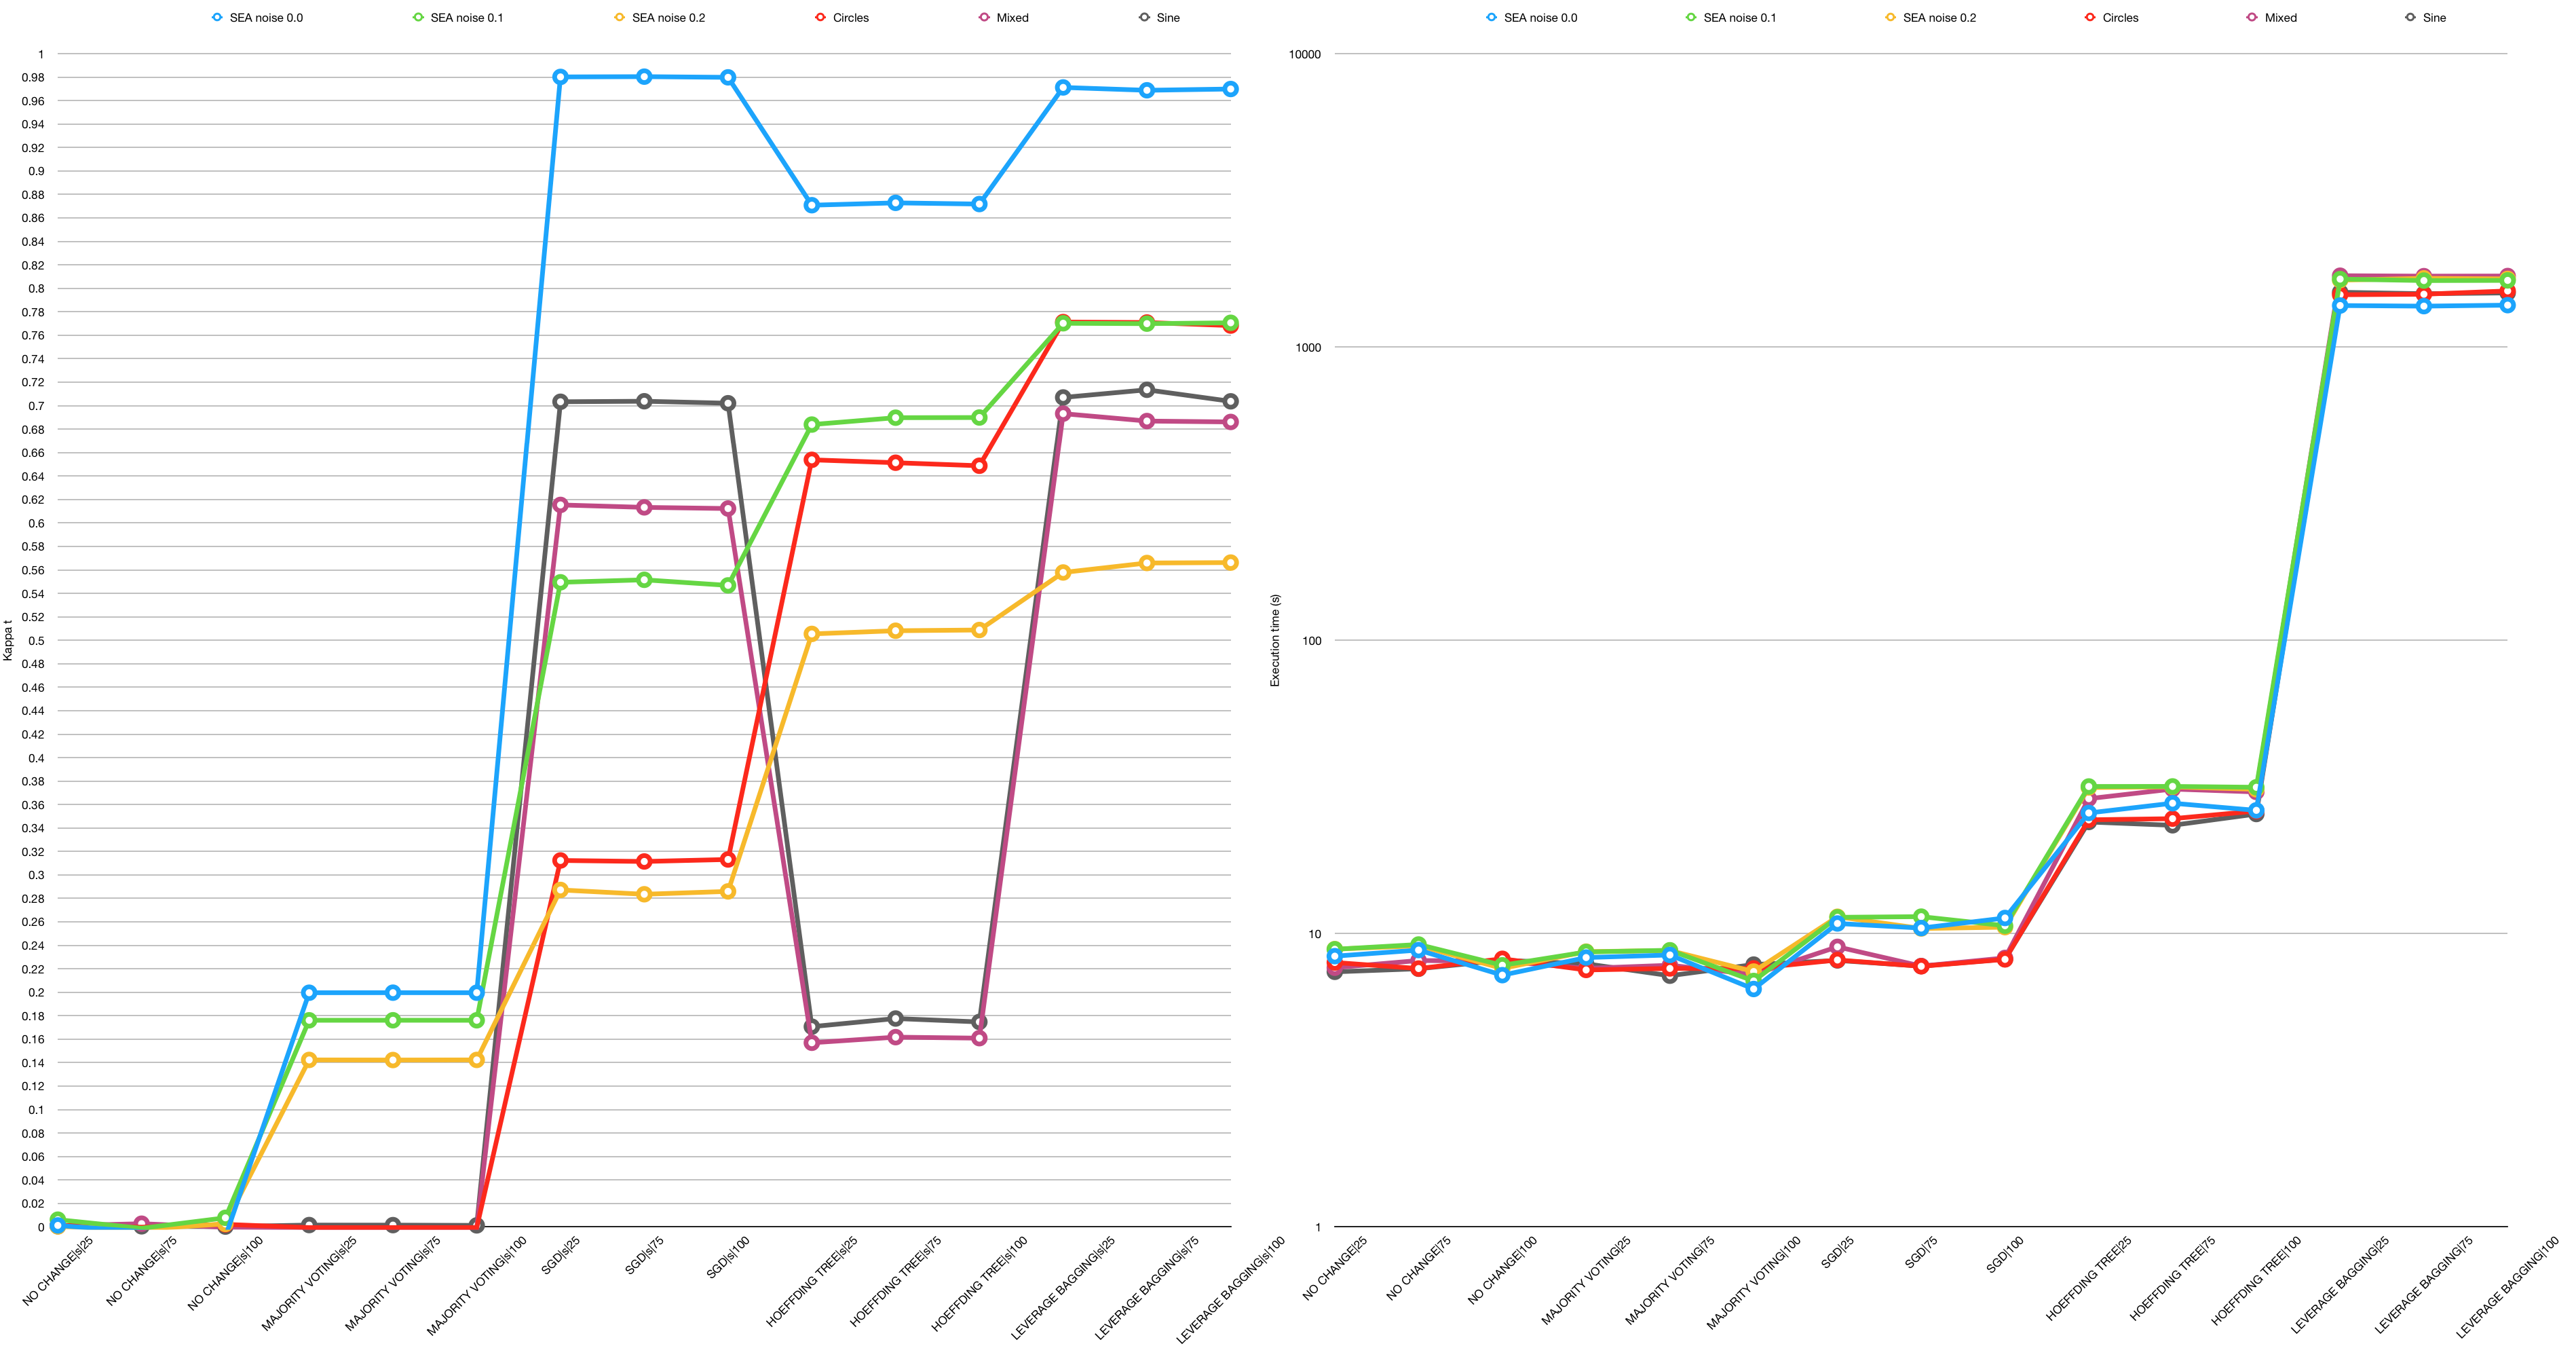
\includegraphics[width=\linewidth]{./images/chapter5/compare_sota}
\caption{\label{fig:raw_compare_sota}$\kappa_t$ and execution times of State of the Art algorithm with varying window sizes}
\end{sidewaysfigure}

For these algorithms, we made sure to use $100\%$ ground truth for the training, sliding windowing and only modified the window size. However, changing the window size did not change the execution times or $\kappa_t$ by much more than $1\%$ or 1 second as can be seen in figure \ref{fig:raw_compare_sota}. For this reason, we chose to keep one example for each algorithm, that ranked better with a given window size than the others. We should note that applying the Friedman test and Nemenyi tests showed that the window size resulted in confirming the null hypothesis that all window sizes led to similar results for each classifier for the no change, majority voting, and SGD classifiers. Therefore, we took the best overall ranking window size. For Hoeffding Trees, a window size of 25 showed a significant statistical difference to 100 but only for the execution time. For Leveraging Bagging, a window size of 25 showed a significant statistical difference to 100 but only for the $\kappa_t$ metric.

The resulting chosen window sizes are as follows: no change (25),  majority voting (25), SGD (75), Hoeffding Tree (25), Leveraging Bagging (25).

We have opted to compare these algorithms to our voting ensemble with six different parameter combinations (1 for each increment of ground truth used, and an additional one using $100\%$ ground truth).


\subsection{Visual comparison}

Finally, we can compare our voting ensemble to the state of the art. Figure \ref{fig:raw_compare_sota_all} shows the raw results, to better visualise how each algorithm, and its parameter combinations affect the data sets that they are trying to model.

\begin{sidewaysfigure}
  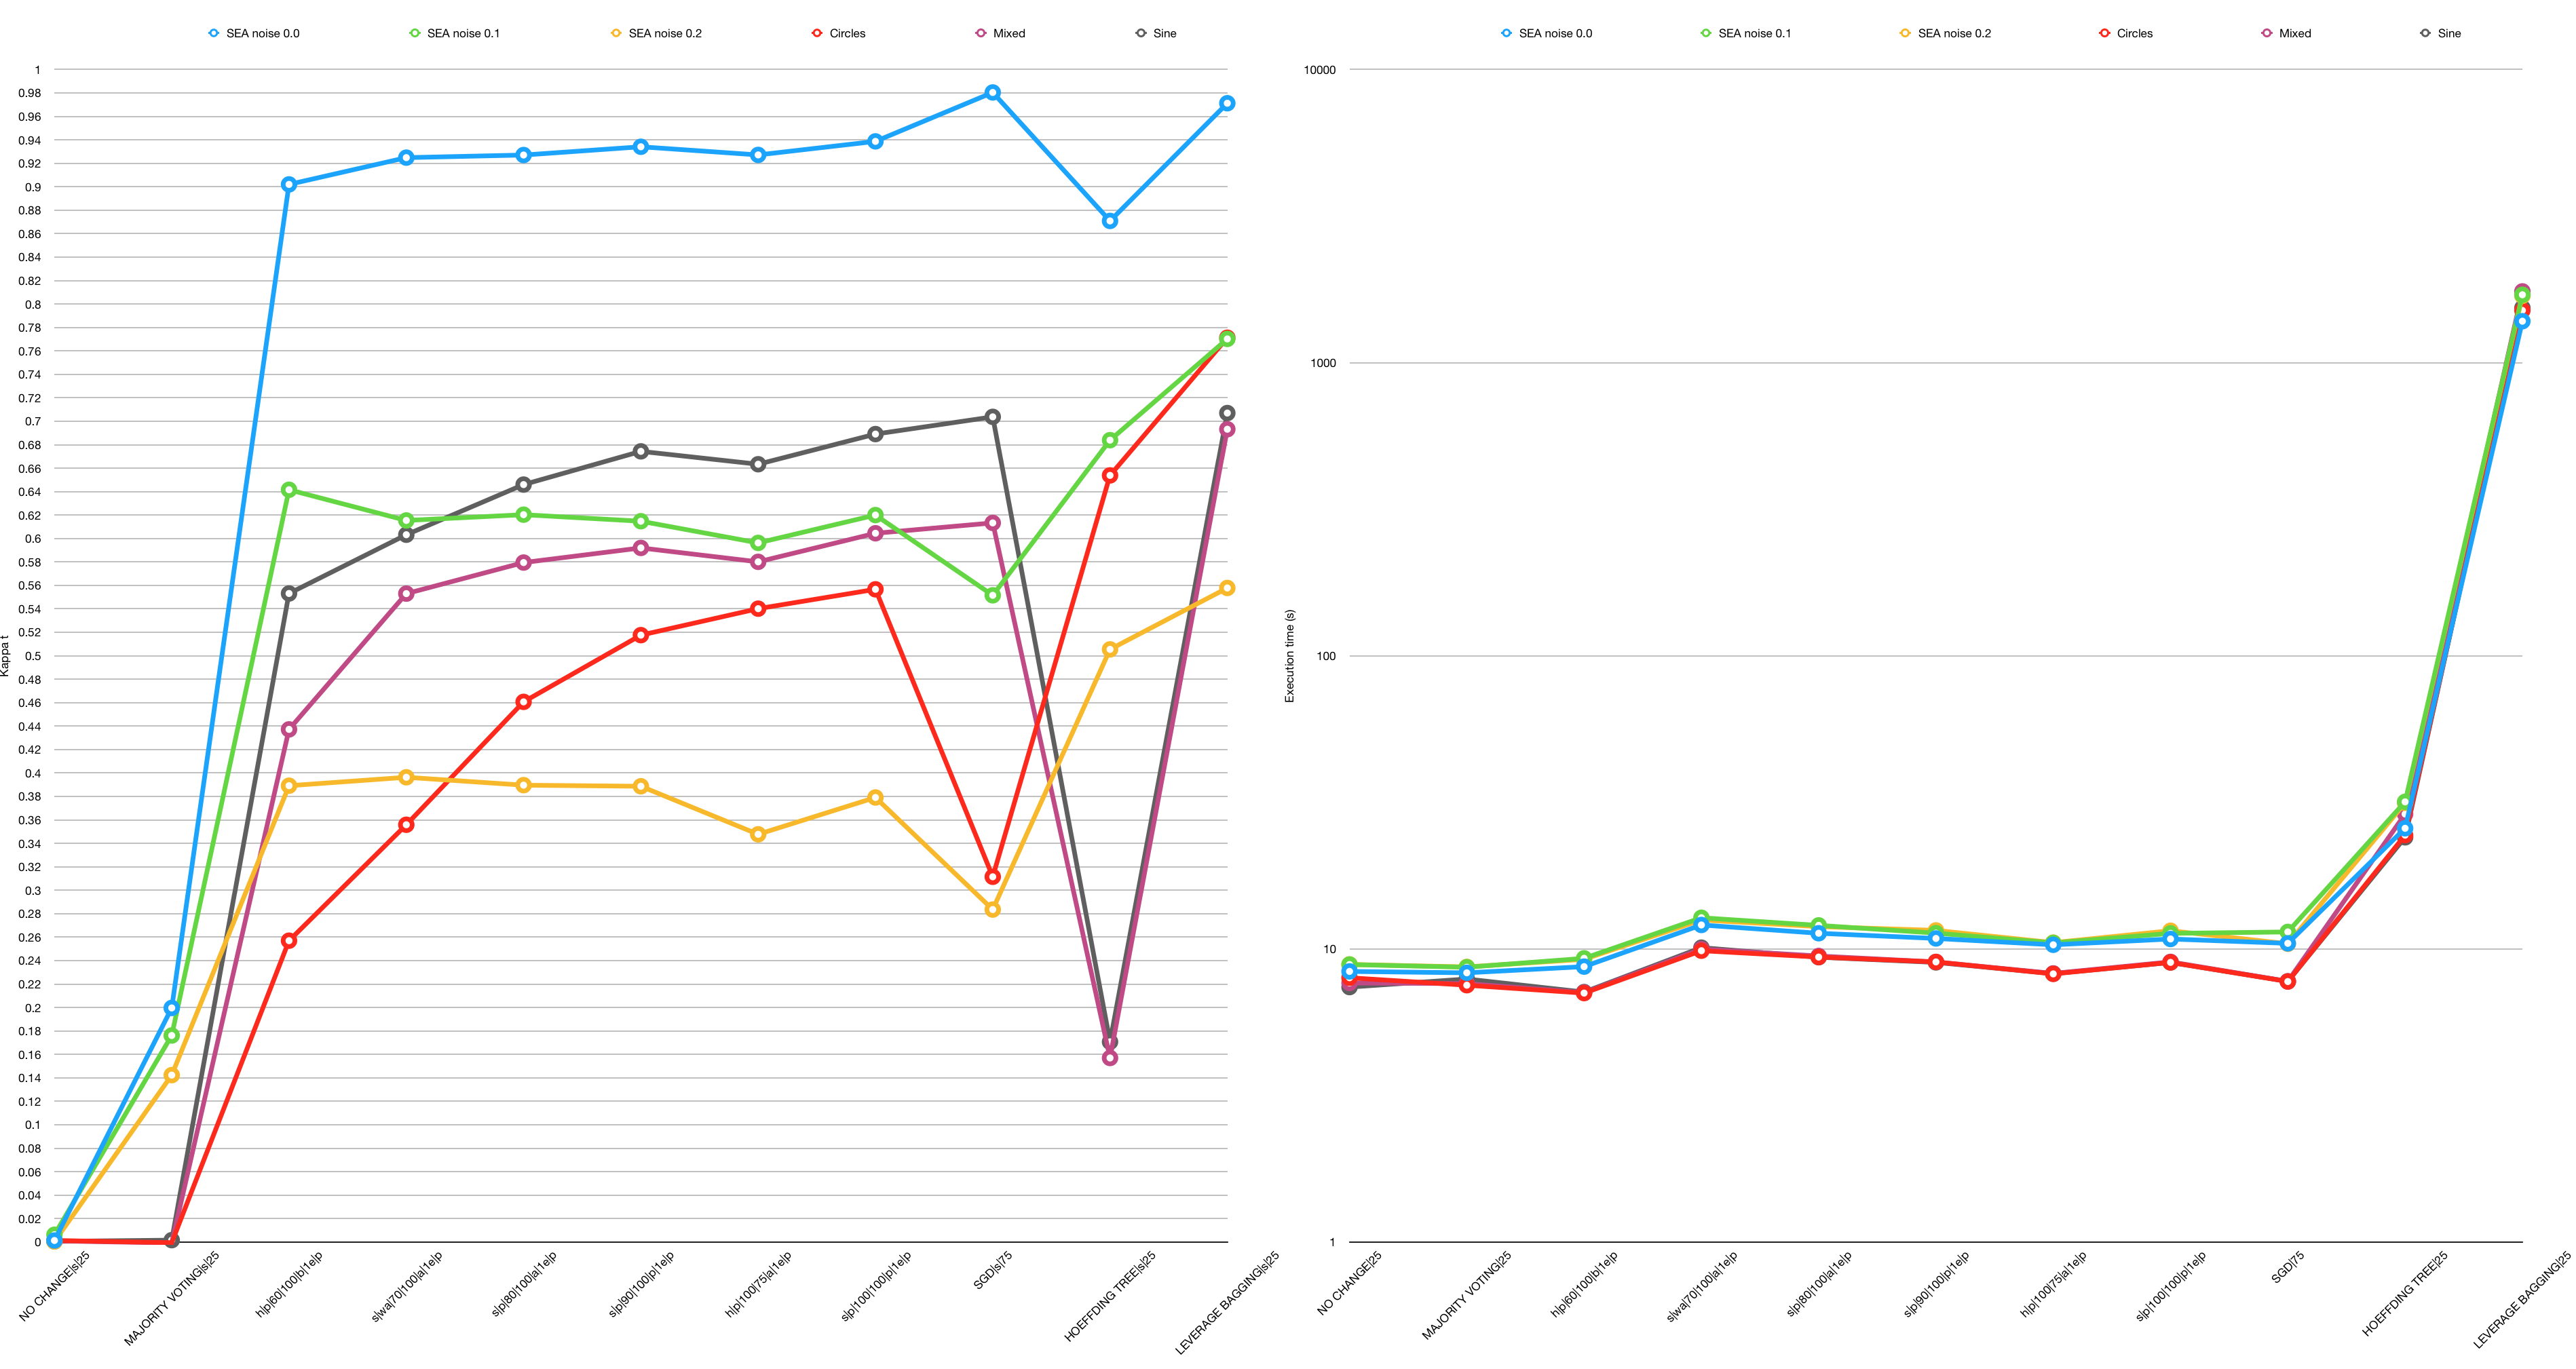
\includegraphics[width=\linewidth]{./images/chapter5/compare_sota_all}
\caption{\label{fig:raw_compare_sota_all}$\kappa_t$ and execution times when comparing our Voting Ensemble to the State of the Art}
\end{sidewaysfigure}

As we can see from these two graphs, Leveraging Bagging (LB) does achieve the best predictive accuracy but the worst execution time. While the difference in predictive accuracy between LB and the other algorithms is noticeable, it is not glaring. However, when it comes to execution time, we were required to use a logarithmic scale to show its run time while also showing the run times of other algorithms. LB takes more than two orders of magnitude longer than the Voting Ensemble, and 1.5 orders of magnitude longer than a Hoeffding Tree (HT). Given that LB is comprised of 10 HTs, it makes perfect sense that LB takes so much longer to run.

However, our findings from the graph do not have the weight of a proper statistical analysis, which follows in the next section.

\subsection{Statistical Analysis}
In this final section, we will test the following two null hypotheses:
\begin{enumerate}
\item all algorithms, with their respective parameters predict classes equally well ($\kappa_t$)
\item all algorithms, with their respective parameters run in an equal amount of time.
\end{enumerate}

\subsubsection{For $\kappa_t$}

We will start with the first, using the $\kappa_t$ metric. Again, the Friedman test was used, with a significance level of 0.05. We found that $p < 2.1\times10^{-23}$, thus rejecting the null hypothesis.
To determine which pairs of algorithms actually differ, we used the post-hoc Nemenyi test, yet again. The results can be seen in figure \ref{fig:sota_compare_all_kappa_nemenyi}, where a lower rank means a better predictive accuracy (a better $\kappa_t$).

\begin{figure}
  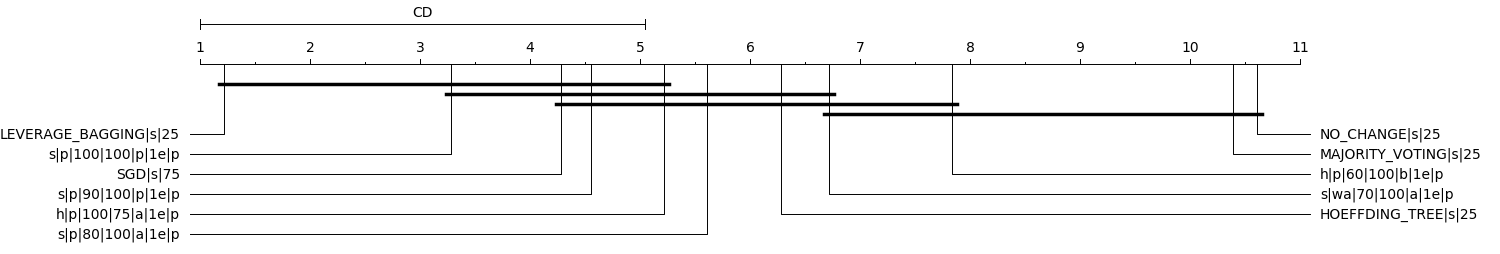
\includegraphics[width=\linewidth]{./images/chapter5/sota_compare_all_kappa_nemenyi}
\caption{\label{fig:sota_compare_all_kappa_nemenyi}Nemenyi graph ranking $\kappa_t$ for various algorithms}
\end{figure}

A Nemenyi graph shows a ranking of algorithms on a scale from 1 to N (typically the number of algorithms compared). A bar labelled critical difference (CD) is shown above the scale, which is the minimum rank length for two algorithms to not show a significant statistical difference in rank. 
Additionally, there may be horizontal bars that link ranked algorithms. Any algorithms that share the same horizontal bar are not significantly statistically different. Pairs of algorithms that are further apart than the CD bar are significantly statistically different.

The graph shows that there is no significant statistical difference between LB, our Voting Ensemble using our best overall parameter combination, an SGD classifier, our Voting Ensemble using our hybrid windowing approach, and our Voting Ensemble using only $80\%$ ground truth when training. This supports the rejection of the null hypothesis for $\kappa_t$. It is also a very good sign, because all of the above-mentioned algorithms were statistically significantly better than a single Hoeffding Tree.

Note that there is a significant statistical difference between both the majority voting and no change classifiers with all algorithms, aside from our Voting Ensemble training with $70\%$ of ground truth or less.

Therefore, this test showed that our Voting Ensemble, using our preferred parameter combinations, did not perform better or worse, statistically speaking, than Leveraging Bagging.

\subsubsection{Considering execution time}

For the final measure, execution time, we use the Friedman test, with a significance level of 0.05. We found that $p < 1.68\times10^{-31}$, thus leaving no doubt as to the rejection of the null hypothesis. The post-hoc Nemenyi test is used to determine which pairs of algorithms differ. The Nemenyi graph is shown in figure  \ref{fig:sota_compare_all_execution_time_nemenyi}, where a lower rank means a lower, thus better, execution time.

\begin{figure}
  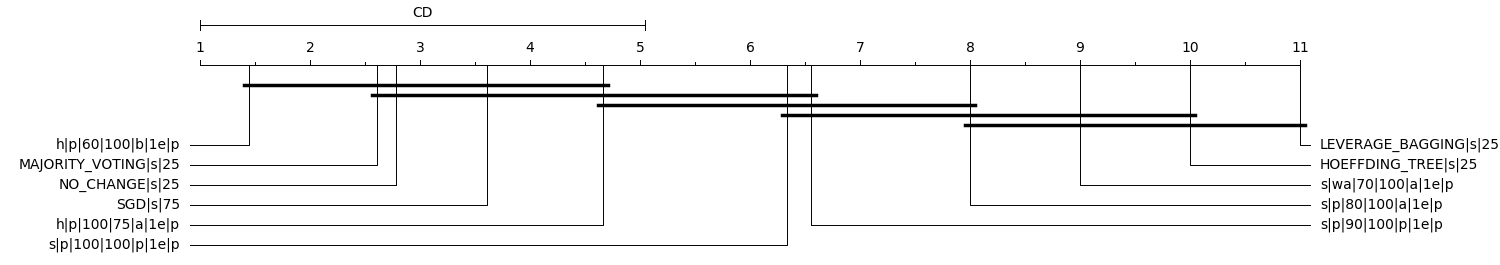
\includegraphics[width=\linewidth]{./images/chapter5/sota_compare_all_execution_time_nemenyi}
\caption{\label{fig:sota_compare_all_execution_time_nemenyi}Nemenyi graph ranking execution times for various algorithms}
\end{figure}

The graph indicates that Leveraging Bagging ranks last, and Hoeffding Trees ranks second last, which is as expected given the raw values that we saw above. 
The graph also shows that there is a significant statistical difference between Leveraging Bagging (the State of the Art algorithm we are comparing), and our Voting Ensemble (except when using $70\%$ or $80\%$ ground truth). Given that Leveraging Bagging runs in over two orders of magnitude longer than our Voting Ensemble, this result is not surprising in the least. It is, however, comforting to have our visual analysis backed by this statistical test.

Therefore, this test statistically showed that our Voting Ensemble runs significantly faster than Leveraging Bagging.

Refer to appendix \ref{section:nemenyi-graphs-statistical-analysis} for additional statistical significance heat-maps and Nemenyi graphs.

\subsection{Discussion}
First of all, our statistical significance tests show that our Voting Ensemble is able to outperform the State of the Art \textit{Leveraging Bagging} algorithm in execution time, and that it is able to perform on par with \textit{Leveraging Bagging} in regards to the $\kappa_t$ measured metric. It also indicated that the predictive performance of our ensemble when trained with only $90\%$ ground truth does not present a statistical significant difference to that of \textit{Leveraging Bagging}. When using a p value of 0.01, however, \textit{Leveraging Bagging}'s predictive performance does not present a difference that is statistically different to those of our ensemble trained on a data set containing only $80\%$ labelled data.

Our algorithm therefore predicts comparably to Leveraging Bagging and brings outstanding time savings in algorithm execution-time, running approximately 160 times faster.

\section{Summary}
A preliminary examination of our results shows that our framework's execution time is, at most, very loosely tied to its predictive accuracy.

An investigation on the impact of each parameter value on the mean of each metric leads us to determine how to roughly maximise $\kappa_t$ or minimise the execution time.
The differences lie with the window type, the batch size, the percentage of labelled data used and, partially, the drift detector count. Our results indicate that using probability voting, one detector per ensemble to detect drifts, and resetting all classifiers when drifts occur leads to better $\kappa_t$ values and a lower execution time. For the batch size, window type, and the drift detector count, it is entirely logical that choosing one value over another would change the execution time as they were, at least partially, implemented as time-saving measures.

The findings above are confirmed, and parameter values that tend to rank well are identified by ranking the parameter combinations for each metric. By examining the paired rankings (time and predictive performance), we propose an alternative parameter combination\footnote{hybrid windowing, probability voting, 100\% ground truth, batch sizes of 75 instances, one drift detector for the ensemble tracking its confidence, and completely resetting the ensemble when drifts are detected} that achieves significant time savings over the one with the best predictive performance, while only reducing $\kappa_t$ by one to four percent.

Our framework runs roughly 160 times faster than the state of the art \textit{Leveraging Bagging} algorithm, and it is comparable in terms of the measured $\kappa_t$ metric. Training with only $90\%$ labelled data does not compromise our framework's predictive accuracy in comparison to that of \textit{Leveraging Bagging}, in that no statistical significant difference is observed. Our results also indicate that the predictive accuracy of our ensemble when training on data sets containing less than 80\% labelled data approaches the traditional threshold for statistical significance, and presents no significant difference when using a p-value of $0.01$.

Practically, this means that our ensemble should definitely be considered when execution time is an important metric, since the predictive performance is comparable to that of Leveraging bagging.